\documentclass[11pt,a4paper,oneside]{book}

\usepackage{booktabs}
\usepackage{multirow}
\usepackage{fancyhdr}
%\usepackage{palatino}
%\usepackage{lmodern} 
\usepackage{newcent} 
\usepackage{verbatim}
\usepackage{amsmath,amsthm}
\usepackage{amssymb}
\usepackage{graphicx}
\usepackage{xcolor,colortbl} 
\usepackage{color}
\usepackage{hyperref}
\usepackage{natbib}
\usepackage{tikz}
\usepackage{caption}
\usepackage{subcaption}
\usepackage{mathtools}
\usepackage[hmargin=1in,vmargin=1in]{geometry}
\usepackage{setspace}

\pagestyle{fancy}
\fancyhead{}
\fancyfoot{}
\fancyfoot[LO,LE]{\thepage}
\fancyfoot[RO,RE]{J. M. McCracken}
\fancyfoot[CO,CE]{{\color{red} rough draft}}
\fancyhead[LE,RO]{\slshape \thesubsection}
\fancyhead[LO,RE]{\slshape \leftmark}

\usetikzlibrary{backgrounds,fit,decorations.pathreplacing,calc,,shadows}

\newenvironment{definition}[1][Definition]{\begin{trivlist}
\item[\hskip \labelsep {\bfseries #1}]}{\end{trivlist}}

\newenvironment{theorem}[1][Theorem]{\begin{trivlist}
\item[\hskip \labelsep {\bfseries #1}]}{\end{trivlist}}

\newcommand{\bra}[1]{\ensuremath{\left\langle#1\right|}}
\newcommand{\ket}[1]{\ensuremath{\left|#1\right\rangle}}
\newcommand{\braket}[2]{\langle #1|#2\rangle}
\newcommand{\ketbra}[2]{|#1\rangle\langle#2|}
\newcommand{\mean}[1]{\langle #1\rangle}
\newcommand{\trace}{\operatorname{Tr}}
\newcommand{\Hcol}{\operatorname{col}}
\newcommand{\Hmat}{\operatorname{mat}}
\newcommand{\parasep}{\begin{center}\rule{35em}{0.1em}\end{center}}
\newcommand{\downedit}{
\begin{center}
\line(1,0){250}
\end{center}
\dotfill
{\color{red} This section needs to be expanded and fixed.}
\dotfill
\begin{center}
$\Downarrow\Downarrow\Downarrow\Downarrow\Downarrow\Downarrow\Downarrow\Downarrow\Downarrow\Downarrow$
\end{center}}
\newcommand{\upedit}{
\begin{center}
$\Uparrow\Uparrow\Uparrow\Uparrow\Uparrow\Uparrow\Uparrow\Uparrow\Uparrow\Uparrow$
\end{center}
\dotfill
{\color{red} This section needs to be expanded and fixed.}
\dotfill
\begin{center}
\line(1,0){250}
\end{center}}
\newcommand{\trustnothing}{
\begin{center}
$\Longleftarrow$\hfill$\Longrightarrow$
\end{center}
\dotfill
{\color{red} {\bf TRUST NOTHING BELOW THIS LINE.}}
\dotfill
\begin{center}
$\Longleftarrow$\hfill$\Longrightarrow$
\end{center}
}

\title{Negative Quantum Channels}
\author{James M McCracken}
\date{\today}

\begin{document}
\maketitle
\tableofcontents
\onehalfspacing

\include{Section1}
\chapter{Complete Positivity}
This chapter will introduce the concept of complete positivity and the operator representation theorem for completely positive operations.  It will be shown that reduced dynamics can always be written as a sum of operators, but only completely positive reduced dynamics can be written as a Kraus operator sum.  We will briefly discuss the claim that complete positivity is a physical requirement of nature, and we will point out some problems with this viewpoint.  This chapter will conclude with the introduction of the negativity, which will be our primary tool for identifying negative channels.

\section{Complete Positivity Definition}
\label{sec:cpDef}

Mathematically, the requirement of complete positivity can be formulated as follows: Consider an extension of $\mathcal{H}^A$ to the space $\mathcal{H}^A\otimes\mathcal{H}^B$.  The map $\Phi^A$ is ``completely positive'' on $\mathcal{H}^A$ if (and only if) $\Phi^A\otimes I_n$ is positive for all such extensions.  Following Choi's formulation \cite{Choi1972,Choi1975}, suppose $\Phi^A(a) \ge 0$ for every $a\ge 0$ and $a\in\mathcal{B}(\mathcal{H}^A)$, then $\Phi^A\otimes I_n $ ,where $I_n$ is the identity matrix of dimension $n$, is called ``n-positive" if $\Phi^A\otimes I_n \ge 0$.  If
\begin{equation}
\Phi^A\otimes I_n \ge 0 \;\forall n\;\;,
\end{equation}
then $\Phi^A$ is called ``completely positive''.  A map that is completely positive is a map that takes a positive operator to another positive operator under any trivial extension.  It should be noted that this definition assumes finite spaces, which is made perfectly clear in the math literature (e.g.\ \cite{Choi1975,Stinespring1955}, but can be a little nebulous in the physics literature (e.g.\ \cite{Benatti2005}) where discussions of complete positivity with (continuous) infinite baths are often conflated with discussions of Markovity in dynamical semigroup methods.  The issues surrounding dynamical semigroup methods will be discussed in Sec.\ \ref{sec:multibath}.

A fundamental (and  very useful) proof due to Choi shows that if $\Phi^A\otimes I_n \ge 0$ when $I_n$ is the same dimension as $\Phi^A$, then $\Phi^A$ is completely positive \cite{Choi1972,Choi1975}.  This result means that complete positivity can be checked just by doubling the dimension of the Hilbert space of the reduced system, which will lead to the construction of a special matrix (called ``Choi's matrix'') to check for complete positivity.

One of the most important properties of completely positive maps is given by the following theorem: 
\begin{theorem}
The {\em representation theorem of quantum operations} states that an operation $\Phi$ that is
\begin{itemize}
\item convex linear, i.e.\ $\Phi\left(\sum_i p_i\rho_i\right)=\sum_ip_i\Phi_m(\rho_i)$ with $\sum_i p_i = 1$ and $p_i\in[0,1]$, 
\item completely positive, i.e.\ $\Phi \otimes I_n \ge 0 \;\forall n$, and
\item trace preserving, i.e.\ $\trace\left(\Phi(\rho)\right)\le\trace\left(\rho\right)$
\end{itemize}
can be written as
\begin{equation}
\label{eqn:opsumform}
\Phi(\rho)  = \sum_k E_{k}\rho E_{k}^\dagger
\end{equation}
where $\rho\in\mathcal{S}(\mathcal{H}^S)$ and 
$$
\sum_k E_{k}^\dagger E_{k}= I\;\;.
$$
Additionally, any map that can be written in the form of Eqn.\ \ref{eqn:opsumform} is completely positive, trace-preserving, and convex linear.
\end{theorem}

Proofs of this theorem can be found in \cite{Breuer2007,Kraus1983}, and discussions of this theorem can be found in most standard quantum information textbooks, including \cite{Nielsen2010} and \cite{Preskill2004}.  This operator sum form of a completely positive map (i.e.\ Eqn.\ \ref{eqn:opsumform}) is referred to as ``Choi's form'', ``Kraus' form'' (or, alternatively the ``Kraus decomposition'' of the operator), or sometimes even ``Sudarshan's form''.   

The Kraus decomposition can be used to describe a completely positive map.  However, the practicality of the decomposition is restricted to finite dimensional system-environment Hilbert spaces.  For systems with high (or infinite) dimensional Hilbert spaces, the Kraus decomposition will lead to an impractically large number of Kraus operators.  Examples of infinite dimensional environments occur quite often in the study of thermodynamics and include heat baths and baths of harmonic oscillators (e.g.\ to model electromagnetic noise in transmission lines).  In such cases, completely positive maps are usually dealt with using dynamical semigroup methods.  Infinite dimensional baths and semigroup methods will be discussed in Sec.\ \ref{sec:multibath}.

\section{Reduced System Evolution as an Operator Sum}
\label{sec:redsysopform}
It is possible to write the reduced dynamics of a system in the Kraus form given some strict assumptions about initial correlations and couplings.  The reduced dynamics can be written out explicitly in terms of the spectral forms of the composite state and evolution to show a general form of the reduced dynamics as a sum of operators.  Applying specific assumptions to this general form will allow the reduced dynamics to be written in the Kraus form introduced in the previous section.

Suppose the time evolution of the reduced state is due to some interaction with the environment, i.e.\
$$
\rho^S(t) = \left((U^{SB}(t))\left(\rho^{S}\right)^\sharp(U^{SB}(t))^\dagger\right)^\flat 
$$
where $\left(\rho^{S}\right)^\sharp$ is the initial state of the composite system and is described (through a spectral decomposition) as
$$
\left(\rho^{S}\right)^\sharp = \sum_i \lambda_i \ketbra{\Psi_i}{\Psi_i}\;\;,
$$
where each $\ket{\Psi_i}\in\mathcal{H}^{SB}$ can be written in terms of the system and bath basis states, i.e.\ 
$$
\ket{\Psi_i} = \sum_{mn} a_{mn}^{(i)} \ket{s_m b_n}\;\;.
$$
The states $\ket{s_m}\in\mathcal{H}^S$ are an orthonormal basis for the reduced system and $\ket{b_n}\in\mathcal{H}^B$ are an orthonormal basis for the bath.  The state of the composite system is then
\begin{eqnarray*}
\left(\rho^{S}\right)^\sharp &=& \sum_i \lambda_i \left(\sum_{mn} a_{mn}^{(i)} \ket{s_m b_n}\right)\left(\sum_{m^\prime n^\prime} a_{m^\prime n^\prime}^{(i)*} \bra{s_{m^\prime} b_{n^\prime}}\right)\\
&=& \sum_{imnm^\prime n^\prime} \lambda_i a_{mn}^{(i)}a_{m^\prime n^\prime}^{(i)*} \ketbra{s_m b_n}{s_{m^\prime} b_{n^\prime}}\\
&=& \sum_{imnm^\prime n^\prime} \lambda_i a_{mn}^{(i)}a_{m^\prime n^\prime}^{(i)*} \left(\ketbra{s_m}{s_{m^\prime}} \otimes \ketbra{b_n}{b_{n^\prime}}\right)\;\;.
\end{eqnarray*}
The unitary evolution of the composite system can also be written in terms of its spectral decomposition as
$$
U^{SB} = \sum_j \nu_j \ketbra{\phi_j}{\phi_j}\;\;,
$$
where each combined state of the system and bath can (again) be written in terms of the system and bath basis states, i.e.
$$
\ket{\phi_j} = \sum_{xy} c_{xy}^{(j)} \ket{s_x b_y}\;\;.
$$
The unitary evolution of the composite system\footnote{Notice that the explicit time dependence of the composite evolution has been dropped from the notation to save space, i.e.\ $U^{SB}(t) \rightarrow U^{SB}$.  However, it should be understood that the state of the reduced system at time $t$ will be described by a unitary evolution $U^{SB}$ which, in general, depends on that time $t$.  The complete formal notation of the decomposition of $U^{SB}$ would include explicit time dependence for all of the coefficients, i.e.\ $\nu_j \rightarrow \nu_j(t)$ and $c_{xy} \rightarrow c_{xy}(t)$.} can then be written as
\begin{eqnarray*}
U^{SB} &=& \sum_{jxyx^\prime y^\prime} \nu_j c_{xy}^{(j)}c_{x^\prime y^\prime}^{(j)*} \ketbra{s_x b_y}{s_{x^\prime} b_{y^\prime}}\\
&=& \sum_{jxyx^\prime y^\prime} \nu_j c_{xy}^{(j)}c_{x^\prime y^\prime}^{(j)*}\left( \ketbra{s_x}{s_{x^\prime}} \otimes \ketbra{b_y}{b_{y^\prime}}\right)\;\;.
\end{eqnarray*}
Hence,
$$
\left(U^{SB}\right)^\dagger = \sum_{okpo^\prime p^\prime} \nu_k^* c_{op}^{(k)*}c_{o^\prime p^\prime}^{(k)} \left(|s_{o^\prime} \rangle\langle s_{o} | \otimes |b_{p^\prime} \rangle\langle b_{p} |\right)\;\;.
$$
The reduced system dynamics are then written down as (Appendix \ref{sec:genreddynamics})
\begin{eqnarray*}
\rho^S (t) &=& \left((U^{SB}(t))\left(\rho^{S}\right)^\sharp(U^{SB}(t))^\dagger\right)^\flat  \\
&=& \sum_{imnm^\prime n^\prime q} \lambda_i a_{mn}^{(i)} a_{m^\prime n^\prime}^{(i)*} \hat{S}_{qn} \ketbra{s_m}{s_{m^\prime}} \hat{S}_{qn^\prime}^\dagger\;\;,
\end{eqnarray*}
where
\begin{eqnarray}
\label{eqn:formalS}
\hat{S}_{qn} &=& \sum_{jxx^\prime} \nu_j c_{xq}^{(j)} c_{x^\prime n}^{(j)*} \ketbra{s_x}{s_{x^\prime}}\\
&=& \left( I\otimes \bra{b_q}\right)U^{SB}\left(I\otimes \ket{b_n}\right)
\end{eqnarray}
and
\begin{eqnarray*}
\hat{S}_{qn^\prime}^\dagger &=& \sum_{koo^\prime} \nu_k^* c_{oq}^{(k)*} c_{o^\prime n^\prime}^{(k)} \ketbra{s_{o^\prime}}{s_{o}}\\
&=& \left( I\otimes \bra{b_{n^\prime}}\right)\left(U^{SB}\right)^\dagger\left(I\otimes \ket{b_q}\right)\;\;.
\end{eqnarray*}

At this point, the evolution of the reduced system is described as
\begin{equation}
\label{eqn:gensumeqn}
\rho^S(t) = \sum_{imnm^\prime n^\prime q} \lambda_i a_{mn}^{(i)} a_{m^\prime n^\prime}^{(i)*} \hat{S}_{qn} \ketbra{s_m}{s_{m^\prime}} \hat{S}_{qn^\prime}^\dagger\;\;.
\end{equation}
This sum is not of the form 
$$
\rho(t) = \sum_q \hat{S}_q \rho \hat{S}_q^\dagger\;\;.
$$
Hence, the general evolution of the reduced system is not necessarily completely positive according to the representation theorem of quantum operations.  It should be noted that the most general form of reduced dynamics is not only not completely positive but also not linear and not unique \cite{Lendi2000,Carteret2008}.  We are, however, assuming linearity throughout for simplicity and to maintain the direct link with standard tomography experiments.   

\chapter{Physical Motivation of Complete Positivity}
\label{sec:physmot}

The argument that all physically reasonable operations are completely positive seems to put strict bounds on the types of operations allowed in nature.  As always, rigorous experiments are required to test the complete positivity assumption of quantum operations, but as far as we are aware, no such experiments have yet been conducted\footnote{It should be made clear that negative channels have already been observed in the lab \cite{Boulant2004}.  However, without the testing of complete positivity assumptions being the focus point of the experiment, such observations are not considered ``rigorous'' for our purposes; i.e.\ they do not provide rigorous validation of a given theory of negative channels.}.  Until such experiments are performed, we are left with a mathematical theory that seems to allow negative channels (as shown above) but argues that such channels are not physically reasonable.  There are plenty of examples in theoretical physics of mathematical models being restricted by physically motivated assumptions.  So, it is important to understand such arguments for complete positivity.

The current arguments for completely positivity as a physical requirement of all quantum operations can be grouped into two categories which will be called the ``total domain argument for complete positivity'' and the ``product state argument for complete positivity''.

\section{Total Domain Argument}
\label{sec:totaldomain}

The thought process behind the total domain argument is as follows: Any known Hilbert space cannot be known to be isolated, i.e.\ given only $\mathcal{H}^A$, it is not possible to rule out the existence of $\mathcal{H}^{AC} = \mathcal{H}^A \otimes \mathcal{H}^C$ where $\mathcal{H}^C$ is some arbitrary Hilbert space.  In fact, it is clear that the system of interest can always be thought of as part of a composite system with a trivial bath.  Empirically and mathematically, having no bath is the same has having a trivial bath with respect to the dynamics of the reduced system.  In both cases, the dynamics of the reduced system are explained completely in terms of the reduced system.

Suppose $\rho$ is the initial state of a two qubit composite system.  Define a state in the composite space as
 \begin{equation}
\rho^\prime = I\otimes\varepsilon\left(\rho\right)\;\;.
\end{equation}
It follows that
\begin{equation}
\label{eqn:ent}
\rho = N\sum_{i,j=0}^1\ketbra{ii}{jj} \rightarrow \rho^\prime = N\mathbf{C}\;\;,
\end{equation}
 where $N$ is the appropriate normalization factor.  If $\rho^\prime$ must be a valid quantum state for any $\rho$, then $\rho^\prime\ge 0$ which implies $\mathbf{C}\ge 0$.  It will be shown later (see Sec.\ \ref{sec:choi}) that $\mathbf{C}\ge 0$ implies $\varepsilon$ must be completely positive.  This is the total domain argument for complete positivity.  It can be seen from Eqn.\ \ref{eqn:ent} why this argument has led to the interpretation of complete positivity as a requirement due to possible entanglement between bipartite subsystems.

The total domain argument for complete positivity seems reasonable at first glance.  If a map is a valid quantum map, then it must take valid density matrices to valid density matrices.  A trivial extension of the map is physically reasonable and must result in a valid quantum map, i.e.\ the trivial extension of the quantum map must also take valid density matrices to valid density matrices.  Therefore, the quantum map must be completely positive.  But, notice that the positivity domain is the domain of states in which a map $\Gamma$ will be positive.  On the positivity domain, $\Gamma$ will take valid initial states to valid final states.  Such a requirement is identical in spirit to the requirement of complete positivity except that it is not extended to states which are not actually created in the lab\footnote{This idea is why the tomography vector is used to define the sharp operation introduced in Section \ref{sec:sharpop}.}. 

\section{Product State Argument}

Complete positivity can be imposed on physical grounds without using the total domain argument.  Some authors instead choose to argue that the reduced system and bath must initially be uncorrelated.  Such a situation will always lead to completely positive reduced dynamics. 

Initial composite states that have no correlation between the reduced system and the bath can be written as a product state, i.e.\
\begin{equation*}
(\rho^S)^\sharp = \rho^S \otimes \rho^B\;\;,
\end{equation*}
where $\rho^S\in\mathcal{S}(\mathcal{H}^S)$ is the initial state of the reduced system and $\rho^B\in\mathcal{S}(\mathcal{H}^B)$ is the initial state of the bath.  It will be shown in Sec.\ \ref{sec:prodstates} that the reduced dynamics are completely positive if the initial composite state is a product state.  

Originally, Kraus used a product state argument defense for the complete positivity assumption in his work, but it should be noted that he was careful to point out that such assumptions may not hold outside of the scattering-type experiments he was considering \cite{Kraus1983}.  

In the quantum information literature, the product state argument is often stated as the necessity of preparation in quantum experiments.  It is true that the reduced system must be prepared and ideal preparations destroy all correlations between the reduced system and the bath.  However, the reduced dynamics will only be completely positive if the preparation procedure leaves the bath in the same state after every preparation of the reduced system over the course of the entire experiment.  

It is not reasonable to assume the preparation procedure has such a feature without evidence.  Recovering the complete positivity requirement with an argument of there being some past composite product state destroys the philosophical advantages of complete positivity. It is equivalent to the remark ``If the dynamics are not completely positive, then you've picked the wrong initial state. Your composite system had an earlier composite state that was uncorrelated.''  How is the experimenter to know when such a time existed for the system?  What evidence does he have that such a time ever existed?  The initial state of the composite system is the state of the composite system when the experiment begins; any other definition becomes too difficult to justify. 

Methods for dealing with negative (i.e.\ not completely positive) dynamics in the lab will be discussed in later sections, but first, there will be some discussion of how to determine complete positivity.

\chapter{Measures of Complete Positivity}

The operator sum representation theorem is the key to the mathematical convenience of completely positive dynamics, and it can be used to prove a few simple conditions.  If the composite dynamics are described by ``local unitaries'' or if the initial composite state has ``zero discord'', then completely positive dynamics are guaranteed.  These proofs are shown below.  Other cases require directly testing the system for complete positivity.

\section{Local Unitary Composite Evolution}

The term ``locally unitary'' composite evolution refers to a composite unitary evolution that is of the form
\begin{equation*}
U^{SB} = U^S \otimes U^B\;\;,
\end{equation*}
where $U^S\in\mathcal{B}(\mathcal{H}^S)$ and $U^B\in\mathcal{B}(\mathcal{H}^B)$.  The reduced dynamics become
\begin{eqnarray*}
\rho^S(t) &=& \left(U^{SB}\left(\rho^{S}\right)^\sharp\left(U^{SB}\right)^\dagger\right)^\flat\\
&=&\left(\left(U^S\otimes U^B\right)\left(\sum_{imnlk} \lambda_i a_{mn}^{(i)} a_{lk}^{(i)*}\ketbra{s_m}{s_l}\otimes \ketbra{b_n}{b_k}\right)\left(U^{S\dagger}\otimes U^{B\dagger}\right)\right)^\flat\\
&=& \sum_{imnlk} \lambda_i a_{mn}^{(i)} a_{lk}^{(i)*} \trace\left(U^B\ketbra{b_n}{b_k} U^{B\dagger}\right) U^S\ketbra{s_m}{s_l} U^{S\dagger}\\
&=& \sum_{imlk} \lambda_i a_{mk}^{(i)} a_{lk}^{(i)*} U^S\ketbra{s_m}{s_l} U^{S\dagger}\\
&=& U^S \rho^S U^{S\dagger}\;\;,
\end{eqnarray*}
where $\{\ket{s_i}\}$ is an orthonormal basis that spans $\mathcal{H}^S$, $\{\ket{b_i}\}$ is an orthonormal basis that spans $\mathcal{H}^B$, 
$$
\trace\left(U^B \ketbra{b_n}{b_k} U^{B\dagger}\right) = \trace\left(\bra{b_n}U^{B\dagger}U^B \ket{b_k}\right) = \trace\left(\braket{b_n}{b_k}\right) = \delta_{nk}
$$
by the cyclic property of the trace and the unitarity of $U^B$, $\lambda_i\in\mathbb{R}\;\forall i$, $\{a_{mn}^{(i)},a_{lk}^{(i)}\}\in\mathbb{C}\;\forall i,m,n,l,k$, and
$$
\rho^S=\left(\left(\rho^{S}\right)^\sharp\right)^\flat=\left(\sum_{imnlk} \lambda_i a_{mn}^{(i)} a_{lk}^{(i)*}\ketbra{s_m}{s_l}\otimes \ketbra{b_n}{b_k}\right)^\flat=\sum_{iml} \lambda_{iml}^\prime \ketbra{s_m}{s_l}\;\;,
$$
with
$$
\lambda_{iml}^\prime = \lambda_i \sum_k  a_{mk}^{(i)} a_{lk}^{(i)*}\;\;.
$$

Any local unitary composite evolution will be completely positive.  Notice that this condition applies to the trivial cases of $U^{SB} = U^S \otimes I$, $U^{SB} = I\otimes U^B$, and $U^{SB} = I\otimes I$ where $I$ is the identity operator. 

The key idea is that local unitary composite evolution will lead to completely positive reduced dynamics independent of the form of the initial composite state. 

\section{Product Composite States}
\label{sec:prodstates}
Initial composite states that have no correlation between the reduced system and the bath can be written as a product state, i.e.\
\begin{equation*}
(\rho^S)^\sharp = \rho^S \otimes \rho^B\;\;,
\end{equation*}
where $\rho^S\in\mathcal{S}(\mathcal{H}^S)$ is the initial state of the reduced system and $\rho^B\in\mathcal{S}(\mathcal{H}^B)$ is the initial state of the bath.  In this situation, the reduced dynamics become
\begin{eqnarray*}
\rho^S(t) &=& \left(U^{SB}(\rho^{S})^\sharp\left(U^{SB}\right)^\dagger\right)^\flat\\
&=&\left(U^{SB}\left(\rho^S\otimes\rho^B\right)\left(U^{SB}\right)^\dagger\right)^\flat\\
&=& \left(U^{SB}\left(\rho^S\otimes\sum_i \lambda_i \ketbra{\psi_i}{\psi_i}\right)\left(U^{SB}\right)^\dagger\right)^\flat\\
&=& \sum_{qi} \lambda_i \hat{S}_{qi} \rho^S \hat{S}^\dagger_{qi}\\
&=& \sum_j E_j \rho^S E_j^\dagger\;\;,
\end{eqnarray*}
where $\rho^B=\sum_i \lambda_i \ketbra{\psi_i}{\psi_i}$ is the spectral decomposition of the (fixed) state of the bath, the operators $\hat{S}_{qi}$ are defined in Eqn. \ref{eqn:formalS}, and the operators $E_j=\sqrt{\lambda_i}\hat{S}_{qi}$ with the index $j$ simply relabelling the double index $qi$.  The reduced system and bath are both classically and quantumly uncorrelated in the above equation, but it is possible to have some correlation in the initial composite state that will still consistently lead to completely positive reduced dynamics (see the next subsection).

One of the simplest ways to force complete positivity in Eqn.\ \ref{eqn:gensumeqn} is to make the initial state of the composite system a product state with a fixed bath.  To that end, assume the system and the bath are initially uncorrelated, and the bath is in an initial state of $|b_\phi\rangle$.  In the derivation of Eqn.\ \ref{eqn:gensumeqn}, this assumption requires $n=n^\prime = \phi$.  The initial state of the reduced system can be found using the decomposition of the composite system as (Appendix \ref{sec:genredstate})
$$
\rho^S = ((\rho^{S})^\sharp)^\flat = \sum_{imm^\prime} \lambda_i a_{m\phi}^{(i)} a_{m^\prime \phi}^{(i)*} \ketbra{s_m}{s_{m^\prime}}\;\;,
$$
and the evolution of the reduced system can now be written as
$$
\rho^S(t) = \sum_{q} \hat{S}_{q\phi} \rho^S \hat{S}_{q\phi}^\dagger\;\;.
$$
The familiar form of the operator sum representation can be recovered with the simple substitution of $\hat{S}_{q\phi} = E_w$, which leads to
$$
\rho^S(t) = \sum_{w} E_{w} \rho^S E_{w}^\dagger\;\;.
$$

Notice that it can be shown explicitly from the definition of $\hat{S}_{q\phi}$ (Appendix \ref{sec:Scomrelation}) that
$$
\sum_q \hat{S}_{q\phi}^\dagger \hat{S}_{q\phi} = I\;\;,
$$
as required by the unit trace requirement on the density matrix, i.e.
\begin{eqnarray}
\trace(\rho^S(t)) &=& 1\\
&=& \trace\left( \sum_{q} \hat{S}_{q\phi} \rho^S \hat{S}_{q\phi}^\dagger \right)\\
&=& \trace\left( \sum_{q} \hat{S}_{q\phi}^\dagger \hat{S}_{q\phi} \rho^S \right)\;\;,
\end{eqnarray}
where, by definition, $\trace(\rho^S) = 1$.

\section{Zero Discord Initial Composite States}
The initial correlations between the reduced system and the bath can be formulated in a information theoretical sense using concepts such as the classical and quantum mutual information\footnote{A discussion of these concepts would be a little off-topic here, but a good introduction can be found in \cite{Zurek2003}, \cite{Zurek2002}, \cite{Ollivier2001}, \cite{Rodriguez2010} and \cite{Rodriguez2008A}.}.  
\begin{definition}
A {\em zero discord} state is a state with only classical correlations.  It is enough to note here that a state with only classical correlations between the subsystems of $\mathcal{H}^X$ and $\mathcal{H}^Y$ can be written in the form \cite{Rodriguez2008}
\begin{equation*}
\rho^{XY} = \sum_i \left(\Pi^X_i\otimes I\right) \rho^{XY} \left(\Pi^X_i\otimes I\right)\;\;,
\end{equation*}
where $\Pi^X\in\mathcal{B}(\mathcal{H}^X)$ is a projector (i.e.\ $\left(\Pi^X\right)^2 = \Pi^X$, $\trace(\Pi^X) = 1$, and $\trace(\Pi^X A) = \bra{\phi}A\ket{\phi}$ with $\Pi^X=\ketbra{\phi}{\phi}$).  
\end{definition}
The state $\rho^{XY}$ will contain no entanglement between the subsystems $\mathcal{H}^X$ and $\mathcal{H}^Y$, only classical correlations\footnote{It is interesting to note that almost all quantum states will have a non-vanishing discord \cite{Ferraro2010}.  The zero discord states discussed here are a special form of the initial composite state that leads to completely positive reduced dynamics, and that fact is the only reason they are of interest to this discussion.}.  This form of the initial composite state would be written as \cite{Rodriguez2008}
\begin{equation*}
\left(\rho^{S}\right)^\sharp = \sum_i \left( \Pi^S_i \otimes I\right) \rho^{SB} \left(\Pi^S_i \otimes I \right) = \sum_i \lambda_i \Pi^S_i \otimes \rho^B_i\;\;,
\end{equation*}
with $\lambda_i\ge 0\;\forall i$, $\sum_i \lambda_i = 1$, $\Pi^S_i=\ketbra{s_i}{s_i}$ where \{$\ket{s_i}$\} is an orthonormal basis of $\mathcal{H}^S$, and $\rho^B_i$ is a valid density operator in $\mathcal{S}(\mathcal{H}^B)$.

This initial composite state will lead to completely positive reduced dynamics.  Consider
\begin{eqnarray*}
\rho^S(t) &=& \left(U^{SB}(\rho^{S})^\sharp\left(U^{SB}\right)^\dagger\right)^\flat\\
&=& \left(U^{SB}\left( \sum_i \lambda_i \Pi^S_i \otimes \rho^B_i \right)\left(U^{SB}\right)^\dagger\right)^\flat\\
&=& \sum_{qi} \lambda_i \hat{S}_{qi} \Pi^S_i \hat{S}^\dagger_{qi}\;\;,
\end{eqnarray*}
where, again, the operators $\hat{S}_{qi}$ are defined in Eqn.\ \ref{eqn:formalS}.  Notice that these operators can be expanded as
\begin{equation*}
\hat{S}_{qi} = \sum_x \hat{S}_{qx} \delta_{xi}\;\;,
\end{equation*}
where $\delta$ is a delta function.  This new operator leads to
\begin{eqnarray*}
\rho^S(t)&=& \sum_{qi} \lambda_i \left( \sum_x \hat{S}_{qx} \delta_{xi}\right) \Pi^S_i \left( \sum_y \hat{S}^\dagger_{qy} \delta_{yi}\right)\\
&=& \sum_{qi} \lambda_i \left( \sum_x \hat{S}_{qx} \delta_{xi}\right) \Pi^S_i \Pi^S_i \Pi^S_i  \left( \sum_y \hat{S}^\dagger_{qy} \delta_{yi}\right)\;\;,
\end{eqnarray*}
where $\Pi_i\Pi_i\Pi_i=\Pi_i^2\Pi_i=\Pi_i^2=\Pi_i$.  The orthogonality of projectors leads to $\Pi_i\Pi_x = \delta_{xi}\Pi_i$ or
\begin{equation*}
\hat{S}_{qx} \delta_{xi} \Pi_i^S = \hat{S}_{qx} \Pi^S_x \Pi^S_i \;\;.
\end{equation*}
This relation leads to
\begin{eqnarray*}
\rho^S(t) &=& \sum_{qi} \lambda_i \left( \sum_x \hat{S}_{qx} \delta_{xi} \Pi^S_i\right) \Pi^S_i \left( \sum_y \Pi^S_i \delta_{yi} \hat{S}^\dagger_{qy} \right)\\
&=& \sum_{qi} \lambda_i \left( \sum_x \hat{S}_{qx} \Pi^S_x \Pi^S_i\right) \Pi^S_i \left( \sum_y \Pi^S_i \Pi^S_y \hat{S}^\dagger_{qy} \right)\\
&=& \sum_{qi} \lambda_i \left( \sum_x \hat{S}_{qx} \Pi^S_x \right)\Pi^S_i \Pi^S_i \Pi^S_i \left( \sum_y \Pi^S_y \hat{S}^\dagger_{qy} \right)\\
&=& \sum_{qi} \lambda_i \left( \sum_x \hat{S}_{qx} \Pi^S_x \right)\Pi^S_i\left( \sum_y \Pi^S_y \hat{S}^\dagger_{qy} \right)\\
&=& \sum_{qi} \lambda_i E_q \Pi^S_i E^\dagger_q\\
&=& \sum_q E_q \rho^S E_q^\dagger\;\;,
\end{eqnarray*}
where 
\begin{equation}
\label{eqn:zdrs}
\rho^S = \left(\left(\rho^{S}\right)^\sharp\right)^\flat=\left(\sum_i \lambda_i \Pi^S_i \otimes \rho^B_i\right)^\flat = \sum_i \lambda_i \Pi_i^S\;\;,
\end{equation}
and $E_q \equiv \sum_m \hat{S}_{qm} \Pi^S_m$.  The basic property of conjugate transposes, $(AB)^\dagger=B^\dagger A^\dagger$, was used in conjunction with the Hermiticity of projectors, i.e.\ $\Pi=\Pi^\dagger$, in the above derivation.  Notice,
$$
\sum_q E_q^\dagger E_q = \sum_{qm} \Pi^S_m \hat{S}^\dagger_{qm} \hat{S}_{qm} \Pi^S_m = \sum_m \Pi^S_m = I\;\;,
$$
where $\sum_q \hat{S}^\dagger_{qm} \hat{S}_{qm} = I$ was explained in the introduction of the $\hat{S}_{qi}$ operators (i.e.\ Eqn.\ \ref{eqn:formalS}).  Hence, by the representation theorem of quantum operations, zero discord initial composite states lead to completely positive reduced dynamics.  Notice that initial composite states with no correlation (i.e.\ product states) are forms of zero discord states.  This result was first shown in \cite{Rodriguez2008A}.

The discord of a quantum state is basis dependent in the sense that it depends on the specific projectors $\Pi^S_i$ used to define the discord.  The proof that zero discord states always lead to completely positive reduced dynamics is similarly basis dependent.  The reduced dynamics are always completely positive for any composite dynamics if the reduced system can be written in the form of Eqn.\ \ref{eqn:zdrs}; i.e.\ the complete positivity of the reduced dynamics in this proof require that the reduced state system be a convex sum of a given complete set of projectors $\{\Pi_i\}$.  In particular, this limitation means that the zero discord result presented here is not very useful for channels defined with tomography vectors.

To see this point, notice that a tomography vector $\vec{\tau}^{\;\sharp}$ might consist of composite states that have zero discord with respect to different projectors, but the reduced dynamics associated to $\vec{\tau}^{\;\sharp}$ will only be completely positive if every reduced state in $\vec{\tau}$ could be written in the zero discord form of Eqn.\ \ref{eqn:zdrs} with respect to the same set of projectors $\{\Pi_i\}$.  However, if every reduced state in $\vec{\tau}$ could be written in this way, then $\vec{\tau}$ would not be a tomography vector (because it would not be a basis for the reduced system).  For example, consider the states of the canonical qubit tomography vector.  Neither $\ketbra{+}{+}$ nor $\ketbra{+_i}{+_i}$ can be written in a zero discord form using $\{\ketbra{0}{0},\ketbra{1}{1}\}$, and similar troubles arise trying to use $\{\ketbra{+}{+},\ketbra{-}{-}\}$ or $\{\ketbra{+_i}{+_i},\ketbra{-_i}{-_i}\}$ as the projector sets for a zero discord form of the states in $\vec{\tau}$.  For this reason, we will not be using the zero discord result for anything beyond noting the result of this section. 

It should be noted that a recent result in the literature (which has turned out to be very popular) makes the claim that a vanishing quantum discord is necessary and sufficient for a map to be completely positive given any composite dynamics \cite{Lidar2009a}.  This result was disputed within the community \cite{Cesar2013,Simon2013}, and the authors of \cite{Lidar2009a} have recently declared the problem to still be open \cite{Dominy2013}. 

\section{Completely Positive Reduced Dynamics Without A Special Form}
The results of the previous subsections spell out situations in which completely positive reduced dynamics are guaranteed:
\begin{itemize}
\item Regardless of initial correlations (i.e.\ for any initial composite state), local unitary composite evolution always lead to completely positive reduced dynamics.
\item Regardless of coupling (i.e.\ for any composite system evolution), initial composite product states always lead to completely positive reduced dynamics.
\end{itemize}
These two situations are not the only situations in which completely positive reduced dynamics arise.  Examples of completely positive and non-completely positive channels that do not fit into either one of these categories will be discussed in detail in later sections.  But, now we will consider more general forms of the reduced dynamics that lead to complete positivity, but that involve conditions on both the correlation and the coupling.

Consider that, by definition, the reduced state of the system is the state of the composite system with the bath ``traced out'', i.e.\
$$
\rho^S_f = \left(\rho^{SB}_f\right)^\flat\;\;,
$$
with $\rho^{SB}\in\mathcal{S}(\mathcal{H}^{SB})$ and $\rho^S\in\mathcal{S}(\mathcal{H}^S)$ and the subscripts mean ``final'' states.  The dynamics of the composite system are defined by the composite unitary evolution and some initial reduced system state $\rho^S$ as
$$
\rho^{SB}_f = U^{SB} \left(\rho^{S}\right)^\sharp \left(U^{SB}\right)^\dagger\;\;.
$$
Making the direct substitution yields,
\begin{equation}
\rho^{S}_f = \left(U^{SB} \left(\rho^{S}\right)^\sharp \left(U^{SB}\right)^\dagger\right)^\flat\;\;.
\end{equation}
Expand the operators as
\begin{equation}
\rho^{SB} = \sum_i \lambda_i x_i^S \otimes y_i^B
\end{equation}
and
\begin{equation}
U^{SB} = \sum_j \nu_j S_j \otimes B_j\;\;,
\end{equation}
where $\rho^{SB}\in\mathcal{S}(\mathcal{H}^{SB})$ and $U^{SB}\in\mathcal{B}(\mathcal{H}^{SB})$ exist in the composite space, $x^S_i,S_j\in\mathcal{B}(\mathcal{H}^S)$ are restricted to the reduced system space, $y^B_i,B_j\in\mathcal{B}(\in\mathcal{H}^B)$ are restricted to the bath space, and $\lambda_i,\nu_j\in\mathbb{C}$.  Notice that $x_i^S$ and $y_i^B$ are not necessarily valid density matrices and $S_j$ and $B_j$ are not necessarily unitary.  This notation can be directly linked to the notation of Sec.\ \ref{sec:redsysopform} by noticing that the above constants are actually products of the constants in that section and the indices $i$ and $j$ above are actually single index labels for the multi-index sums of that section.  The operators in the above sums are not necessarily unique, orthonormal, or a basis.  The above notation is just a convenient shorthand for the more cumbersome notation of Sec.\ \ref{sec:redsysopform}.  In this new notation, the derivation becomes
\begin{eqnarray}
\label{eqn:notationref}
\rho^S_f &=& \left( \left( \sum_j \nu_j S_j\otimes B_j\right)\left( \sum_i \lambda_i x_i^S\otimes y_i^B\right)\left(\sum_k \nu_k^* S_k^\dagger \otimes B_k^\dagger\right)\right)^\flat\\
&=& \sum_{ijk} \lambda_i \nu_j \nu_k^* \trace\left(B_j y_i^B B_k^\dagger\right) S_j x_i^S S_k^\dagger\\
&=& \sum_{ijk} \lambda_i \alpha_{ijk} \bar{S}_j x_i^S \bar{S}_k^\dagger\;\;,
\end{eqnarray}
with $\alpha_{ijk} = \trace\left(B_j y_i^B B_k^\dagger\right)$, $\bar{S}_j = \nu_j S_j$, and $\bar{S}_k^\dagger = \nu_k^* S_k^\dagger$.  

This description of the reduced system dynamics is always true, but it is not always completely positive.  By the representation theorem, if these reduced dynamics were completely positive, then they should have a Kraus operator sum form.  The question of complete positivity is
\begin{equation}
\label{eqn:cpquestion}
\sum_x E_x \rho^S E_x^\dagger \overset{?}{=} \sum_{ijk} \lambda_i \alpha_{ijk} \bar{S}_j x_i^S \bar{S}_k^\dagger\;\;,
\end{equation}
where $E_x\in\mathcal{B}(\mathcal{H}^S)$ is some arbitrary operator on the reduced system obeying the condition $\sum_x E_x^\dagger E_x = I$, and the initial state of the reduced system is
\begin{equation}
\rho^S = \left(\left(\rho^{S}\right)^\sharp\right)^\flat \;\;.
\end{equation}
The reduced dynamics are completely positive when $\exists\;E_x$ such that the equality of Eqn.\ \ref{eqn:cpquestion} is satisfied.  So, attempting to find such an $E_x$ can be seen as a tool for determining the complete positivity of the reduced dynamics.

We will consider the results that have already been discussed to show some quick examples of trying to rewrite the general form of the reduced dynamics in a Kraus form to determine complete positivity.  If $y_i^B = \rho^B = \ketbra{\phi_f}{\phi_f}\;\forall\;i$ with $\rho^B\in\mathcal{S}(\mathcal{H}^B)$, then 
$$
\alpha_{ijk} = \alpha_{jk} = \trace\left(B_j \rho^B B_k^\dagger\right) = \sum_x \bra{\phi_x}B_j \ketbra{\phi_f}{\phi_f} B_k^\dagger\ket{\phi_x}
$$ 
where $\{\ket{\phi_x}\}$ is an orthonormal basis of $\mathcal{H}^B$ and $\ket{\phi_f}$ is some fixed state of the bath.  In this case, Eqn.\ \ref{eqn:cpquestion} is satisfied with 
$$
E_x = \sum_j \sqrt{\bra{\phi_x}B_j \ket{\phi_f}} \bar{S}_j
$$
and
$$
E_x^\dagger = \sum_k \sqrt{\bra{\phi_x}B_k \ket{\phi_f}} \bar{S}_k\;\;.
$$
This result is just the already proven statement that the reduced dynamics are completely positive, independent of the composite dynamics, if the bath is in some fixed pure state. This case falls under the second bullet point at the beginning of this section.

If the composite dynamics can be written in local unitary form, then $U^{SB} = U^S\otimes U^B$ with $U^S\in\mathcal{B}(\mathcal{H}^S)$ and $U^B\in\mathcal{B}(\mathcal{H}^B)$, both of which must be unitary because $U^{SB}$ is unitary.  The bath modifier term in the reduced dynamics then becomes
$$
\alpha_{ijk} = \alpha_{i} = \trace\left(U^B y_i^B (U^B)^\dagger\right) = \trace\left((U^B)^\dagger U^B y_i^B \right) = \trace\left(y_i^B\right)
$$
by the cyclic property of the trace.  The initial reduced system state would be
$$
\rho^S = \left(\rho^{SB}(t)\right)^\flat = \left(\sum_i \lambda_i x_i^S \otimes y_i^B\right)^\flat = \sum_i \lambda_i \alpha_i x_i^S \;\;,
$$
and Eqn.\ \ref{eqn:cpquestion} would be satisfied with $E_x = \sum_j \bar{S}_j$ and $E_x^\dagger = \sum_k \bar{S}_k^\dagger$ where there is only one term in the sum over $x$.  This result is the statement that local unitary composite dynamics lead to complete positivity for any initial composite state.  This case is the first bullet point at the beginning of this section.

In a more general case, Eqn.\ \ref{eqn:cpquestion} will be satisfied if $\alpha_{ijk} = \kappa$, where $\kappa\ge 0$ is some constant, with $E_x = \sqrt{\kappa} \sum_j \bar{S}_j$ and $E_x^\dagger = \sqrt{\kappa}\sum_k \bar{S}_k^\dagger$.  
\begin{example}
Consider again the qubit channel with a qubit bath and define the composite dynamics as\footnote{These composite dynamics are the famous controlled NOT gate.  This gate will be discussed in much more detail in later sections.}
$$
U^{SB} = \frac{1}{2}\left(\sigma_0\otimes\sigma_0 + \sigma_0\otimes\sigma_1 - \sigma_3\otimes\sigma_1 + \sigma_3\otimes\sigma_0\right)\;\;.
$$
If the initial composite state is
$$
\rho^{SB} = \rho\otimes \left(R\rho R^\dagger\right)
$$
where $\rho$ is some valid density matrix and 
$$
R = \begin{pmatrix}
\cos{\phi}&-\sin{\phi}\\
\sin{\phi}&\cos{\phi}
\end{pmatrix}\;\;,
$$
then the reduced dynamics become
\begin{eqnarray*}
\rho^S_f &=& \frac{1}{4}\left( \left( \sigma_0\otimes\sigma_0 + \sigma_0\otimes\sigma_1 - \sigma_3\otimes\sigma_1 + \sigma_3\otimes\sigma_0\right)\right.\\
& &\;\;\;\;\;\;\;\;\;\;\;\;\;\left.\left( \rho\otimes \left(R\rho R^\dagger\right)\right)\left(\sigma_0\otimes\sigma_0 + \sigma_0\otimes\sigma_1 - \sigma_3\otimes\sigma_1 + \sigma_3\otimes\sigma_0\right)\right)^\flat\\
&=& \frac{1}{4}\left( \alpha_{00} \left(\sigma_0\rho\sigma_0 + \sigma_0\rho\sigma_3 + \sigma_3\rho\sigma_0 + \sigma_3\rho\sigma_3\right)\right.\\
& &\;\;+ \alpha_{01} \left( \sigma_0\rho\sigma_0 - \sigma_0\rho\sigma_3 + \sigma_3\rho\sigma_0 - \sigma_3\rho\sigma_3\right)\\
& &\;\; + \alpha_{10}\left( \sigma_0\rho\sigma_0 +\sigma_0\rho\sigma_3 - \sigma_3\rho\sigma_0 - \sigma_3\rho\sigma_3 \right) \\
& &\;\;\left.+ \alpha_{11}\left( \sigma_0\rho\sigma_0 - \sigma_0\rho\sigma_3 - \sigma_3\rho\sigma_0 +\sigma_3\rho\sigma_3 \right) \right)\;\;,
\end{eqnarray*}
where the bath modifier terms are
\begin{eqnarray*}
\alpha_{00} &=& \trace\left( \sigma_0 R \rho R^\dagger \sigma_0 \right) = 1\;\;,\\
\alpha_{11} &=& \trace\left( \sigma_1 R \rho R^\dagger \sigma_1 \right) = 1\;\;,\\
\alpha_{01} &=& \trace\left( \sigma_0 R \rho R^\dagger \sigma_1 \right) = \trace\left( R^\dagger \sigma_1 R \rho \right)
\end{eqnarray*}
and
$$
\alpha_{10} = \trace\left( \sigma_1 R \rho R^\dagger \sigma_0 \right) = \trace\left( R^\dagger \sigma_1 R \rho \right) = \alpha_{01}
$$
by the unitarity of $R$, the cyclic property of the trace, the unit trace condition of $\rho$, and the nice property of the Pauli matrices that $\sigma_m\sigma_n = \delta_{mn} \sigma_0 + \delta_{(m+n)1}\sigma_1$ when $m,n=0,1$.  Plugging this back into the reduced dynamics yields
\begin{eqnarray*}
\rho^S_f &=& \frac{1}{4}\left( \left(\sigma_0\rho\sigma_0 + \sigma_0\rho\sigma_3 + \sigma_3\rho\sigma_0 + \sigma_3\rho\sigma_3\right)\right.\\
& &\;\;+ \alpha_{01} \left( \sigma_0\rho\sigma_0 - \sigma_0\rho\sigma_3 + \sigma_3\rho\sigma_0 - \sigma_3\rho\sigma_3\right)\\
& &\;\; + \alpha_{01}\left( \sigma_0\rho\sigma_0 +\sigma_0\rho\sigma_3 - \sigma_3\rho\sigma_0 - \sigma_3\rho\sigma_3 \right) \\
& &\;\;\left.+ \left( \sigma_0\rho\sigma_0 - \sigma_0\rho\sigma_3 - \sigma_3\rho\sigma_0 +\sigma_3\rho\sigma_3 \right) \right)\\
&=& \frac{1}{4}\left( 2 \left(\sigma_0\rho\sigma_0 + \sigma_3\rho\sigma_3\right)+ 2\alpha_{01} \left( \sigma_0\rho\sigma_0 - \sigma_3\rho\sigma_3\right)\right)\;\;.
\end{eqnarray*}
Notice,
$$
\sigma_0\rho\sigma_0 \pm \sigma_3\rho\sigma_3 = \left(\sigma_0\pm\sigma_3\right)\rho\left(\sigma_0\pm\sigma_3\right) \mp \sigma_0\rho\sigma_3 \mp \sigma_3\rho\sigma_1\;\;,
$$
which implies
\begin{eqnarray*}
\rho^S_f &=& \frac{1}{2}\left( \left(\left(\sigma_0+\sigma_3\right)\rho\left(\sigma_0+\sigma_3\right) - \sigma_0\rho\sigma_3 - \sigma_3\rho\sigma_0\right)\right.\\
& &\;\;\left. + \alpha_{01} \left( \left(\sigma_0-\sigma_3\right)\rho\left(\sigma_0-\sigma_3\right) + \sigma_0\rho\sigma_3 + \sigma_3\rho\sigma_0\right)\right)\\
&=& \ketbra{0}{0}\rho\ketbra{0}{0} + \alpha_{01} \ketbra{1}{1}\rho\ketbra{1}{1} - \frac{[\rho,\sigma_3]}{2}(\alpha_{01}-1)
\end{eqnarray*}
where the commutator of two matrices $A$ and $B$ is $[A,B] = AB-BA$ and the computational basis projectors of $\ketbra{0}{0}$ and $\ketbra{1}{1}$ are used to simplify the notation.  This form of the reduced dynamics makes it clear that the dynamics are completely positive if $\alpha_{01}=1$; i.e.\ Eqn.\ \ref{eqn:cpquestion} will be satisfied with $E_1 = \ketbra{0}{0}$ and $E_2 = \ketbra{1}{1}$ if $\alpha_{01}=1$.  

Notice that the bath modifier term $\alpha_{01}$ contains the product
$$
R^\dagger\sigma_1R = \begin{pmatrix}
\sin{\left(2\phi\right)}&\cos{\left(2\phi\right)}\\
\cos{\left(2\phi\right)}&-\sin{\left(2\phi\right)}
\end{pmatrix}\;\;,
$$
which is not equal to $\sigma_0$ for any $\phi$.  Also notice that $R^\dagger\sigma_1R$ is not trace-preserving.  These observations help point out that the condition of $\alpha_{01} = 1$ is a condition on both $R$ and the initial state $\rho$.  For example, if $\rho$ is the computational ground state, i.e.\ $\rho = (\sigma_0+\sigma_3)/2$, and $\phi=\pi/4$, then $R^\dagger\sigma_1R(\sigma_0+\sigma_3)/2 = (\sigma_3+\sigma_0)/2$ and $\alpha_{01}=1$.  It can be shown that these reduced dynamics are completely positive if $\phi=\pi/4$ using Choi's theorem, which will be introduced in the next section.  It is interesting to notice, however, that such a conclusion is difficult to make using only Eqn.\ \ref{eqn:cpquestion} as the test for complete positivity.
\end{example}

This example illustrates the fact that if the composite dynamics or initial composite state are not in the previously discussed specific forms, then whatever form the initial composite state takes will put restrictions on the possible forms of the composite dynamics that guarantee completely positive reduced dynamics, and vice versa.  These results rely on the Kraus representation theorem of completely positive maps, but the next section will introduce another way of determining the complete positivity of a channel.

\section{Choi's Matrix}
\label{sec:choi}

Suppose an experiment is conducted and the map describing the dynamics is not completely positive.  How can an experimenter understand the lack of complete positivity?

The first step is to quantify the degree to which the complete positivity requirement for a map is not met.  Consider a matrix defined as
$$
C = \left(I \otimes \epsilon\right)\sum_{ij} \ketbra{i}{j} \otimes \ketbra{i}{j} = \sum_{ij} \ketbra{i}{j} \otimes \epsilon\left( \ketbra{i}{j} \right)
$$
for some reduced dynamics $\epsilon$ where $\ketbra{i}{j}$ is the matrix of all zero entries with a 1 in the $ij$th position.  A proof due to Choi \cite{Choi1975} states that the map $\epsilon$ is completely positive if and only if $C$ is positive semi-definite\footnote{Notice $\ketbra{i}{j}\otimes \ketbra{i}{j}$ looks like a maximally entangled state.  This notation is used to describe Choi's matrix as the application of the map $\epsilon$ to half of a maximally entangled state.  Leung \cite{Leung2003} outlines a method of performing process tomography based on Choi's proof and a similar logic.}.  

The block diagonal of Choi's matrix consists of $\epsilon$ acting on valid states, but the rest of Choi's matrix must be found by tomography.  As such, $C$ can be written using a constructor on some tomography vector $\vec{\tau}$, i.e.\
$$
C = \mathbf{C}\odot\vec{\tau}(t) = \mathbf{C}\odot\epsilon\left(\vec{\tau}\right),
$$
where the constructor notation was introduced in Sec.\ \ref{sec:notation}.  The map $\epsilon$ was introduced in Sec.\ \ref{sec:map}, and in that section it was pointed out that $\epsilon$ is linear and Hermitian preserving.   These conditions on $\epsilon$ imply that $C$ is Hermitian \cite{Choi1975,Shaji2005}.

The spectral decomposition of $C$ is assured by the Hermiticity; hence,
$$
\mathbf{C}\odot\epsilon(\vec{\tau}) = \sum_r \Lambda_r \ketbra{\Psi_r}{\Psi_r}\;\;,
$$
where $\Lambda_r$ and $\ket{\Psi_r}$ are the eigenvalues and eigenvectors of $C$.  It follows that 
$$
\epsilon\;\;\mathrm{is\ completely\ positive}\Leftrightarrow\Lambda_r\ge 0\;\forall r\;\;.
$$  

Choi's matrix is a common method for testing the complete positivity of tomography data in an experiment, and it extends the concept of complete positivity beyond the operator representation theorem.  Choi's matrix will be the foundation of a quantification of the lack of complete positivity of a channel.  This quantity will be called the negativity.

Before discussion turns to the negativity, a nice relationship between Choi's matrix and the Kraus decomposition needs to be addressed.  Given a superoperator representation of a channel as
$$
S = \mathbf{S}\odot\epsilon(\vec{\tau})\;\;,
$$
the action of the channel on an arbitrary state $\rho_i$ is
$$
\Hmat\left(S\Hcol\left(\rho_i\right)\right) = \rho_f\;\;.
$$
These concepts were introduced in Sec.\ \ref{sec:tomo}.  Given an operator sum form representation of the channel as
$$
\rho_f = \sum_j c_j A_j \rho_i A_j^\dagger\;\;,
$$
it can be shown ``by simple index gymnastics'' \cite{Havel2003} that
$$
S = \sum_j c_j A_j^*\otimes A_j\;\;,    
$$
where $c_j\in\mathbb{C}$ and $A_j^*$ is the complex conjugate of $A_j$.  The definition of Choi's matrix yields, for example in the single qubit case,
$$
C = \mathbf{C}\odot\epsilon(\vec{\tau}) =  \sum_{ij} \ketbra{i}{j} \otimes \epsilon\left( \ketbra{i}{j} \right) = \left(\begin{array}
{c|c} \epsilon(\ketbra{0}{0})&\epsilon(\ketbra{0}{1})\\
\hline
\epsilon(\ketbra{1}{0})&\epsilon(\ketbra{1}{1})
\end{array}\right)\;\;,
$$
which is a 4$\times $4 matrix.  The eigenvectors of $C$ are vectors that can be stacked into matrices as
$$
\Hmat(\ket{\Psi_r})\;\;.
$$
Notice that a superoperator $S$ can be constructed from $C$ as \cite{Havel2003}
$$
S = \sum_r \Lambda_r \Hmat(\ket{\Psi_r})^*\otimes \Hmat(\ket{\Psi_r})\;\;,
$$
from which the operator sum representation follows from the action of $S$ on some arbitrary state $\rho_i$ as
\begin{eqnarray*}
\Hmat\left(S\Hcol(\rho_i)\right) &=& \Hmat\left(\left(\sum_r \Lambda_r \Hmat(\ket{\Psi_r})^*\otimes \Hmat(\ket{\Psi_r})\right)\Hcol(\rho_i)\right)\\
 &=& \sum_r \Lambda_r \Hmat(\ket{\Psi_r})\rho_i \Hmat(\ket{\Psi_r})^\dagger\;\;.
\end{eqnarray*}

Choi's matrix is constructed from some tomography experiment characterized by a tomography vector $\vec{\tau}$ and is related to the superoperator representation of the channel through a re-stacking procedure.  In fact, the Choi representation of a channel was originally introduced by Sudarshan and Jordan in 1961 \cite{Sudarshan1961} as a re-stacking of the superoperator representation.  Choi's work in 1975 \cite{Choi1975} cemented the relationship between the Choi matrix representation of a channel and complete positivity, but it was not the first introduction of the idea despite the naming conventions for these matrices.

Define a restacking procedure $(\cdot)^R$ such that
\begin{eqnarray*}
C^R &=& \left(\mathbf{C}\odot\epsilon(\vec{\tau})\right)^R \\
&=& \left(\sum_{ij}^n \ketbra{i}{j} \otimes \epsilon\left( \ketbra{i}{j} \right)\right)^R\\
&=& S \\
&=& \left(\Hcol\left( \epsilon\left( \ketbra{0}{0} \right)\right) \cdots \Hcol\left( \epsilon\left( \ketbra{n}{n} \right)\right) \right)
\end{eqnarray*}
for some Choi matrix $C$ and superoperator representation $S$ of a channel characterized by a tomography vector $\vec{\tau}$ and the reduced dynamics $\epsilon$.  
\begin{example}
Given a single qubit Choi matrix
$$
T = \begin{pmatrix}
a  &b  &c  &d\\
b^*&e  &f  &g\\
c^*&f^*&h  &j\\
d^*&g^*&j^*&k
\end{pmatrix}   
$$
the superoperator is found as
$$
T^R = \begin{pmatrix}
a  &c^*&c  &h\\
b^*&d^*&f  &j^*\\
b  &f^*&d  &j\\
e  &g^*&g  &k
\end{pmatrix}\;\;.
$$
\end{example}
Such an operation is an involution, i.e.\
$$
C = S^R = (C^R)^R\;\;,
$$
which can be seen clearly in the above example.

The Choi representation of a channel can be used to find the output state similar to the way the superoperator representation might be used; i.e. \cite{Paris2004}\
$$
\Hmat\left(S\Hcol(\rho_i)\right) = \rho_f = \trace_S\left(C\left(\rho_i^T\otimes I\right)\right)
$$
where $S$ and $C$ are superoperator and Choi representations (respectively) of the same channel, $\rho_i,\rho_f\in\mathcal{S}(\mathcal{H}^S)$ are the initial and final states of the reduced system, $I$ is the identity operator of the same dimension as $\rho_{i}$, $\trace_S$ is the partial trace over the reduced system, and $\rho^T$ is the transpose of $\rho$.  

Any channel that can be tomographically characterized will have a Choi matrix representation, hence any such channel will have a operator sum form and superoperator representation defined in terms of the eigenvectors of the Choi matrix.  Notice that if the channel is completely positive and has a Choi matrix $C=\sum_r \Lambda_r \ketbra{\Psi_r}{\Psi_r}$, then Kraus operators can be defined as
$$
A_r = \sqrt{\Lambda_r} \Hmat(\ket{\Psi_r})\;\;,
$$
and the action of the channel on an arbitrary state $\rho_i$ would have the Kraus sum form of
$$
\rho_f = \sum_r A_r \rho_i A_r^\dagger\;\;,
$$
with $\sum_r A_r^\dagger A_r = \sum_r \Lambda_r \Hmat(\ket{\Psi_r})^\dagger \Hmat(\ket{\Psi_r}) = I$ \cite{Havel2003}.

When the above form is derived from Choi's matrix, it is called the ``canonical Kraus representaion'' of the channel.  The eigendecomposition of Choi's matrix is not unique, from which follows the non-uniqueness of the Kraus representation.  

Any channel $\epsilon$ with a Choi representation $C$ can be written in an operator sum form as
$$
\epsilon\left(\rho\right) = \sum_r \Lambda_r \left(\Hmat\left(\ket{\Psi_r}\right)\right)\rho\left(\Hmat\left(\ket{\Psi_r}\right)\right)^\dagger = \sum_r \Lambda_r B_r \rho B_r^\dagger
$$
where \{$\Lambda_r$\} are eigenvalues of $C$, \{$\ket{\Psi_r}$\} are eigenvectors of $C$, $B_r = \Hmat\left(\ket{\Psi_r}\right)$, and $\rho$ is some arbitrary reduced system initial state.  If $\Lambda_r\ge 0$ for all $r$, then this sum reduces to the Kraus representation as shown above.  If, however, $\Lambda_r<0$ for some $r$, then the operator sum can be written as
$$
\epsilon\left(\rho\right) = \left(\;\sum_{r\in R} \Lambda_r B_r \rho B_r^\dagger\right) - \left(\;\sum_{k\in K} |\Lambda_k| B_k \rho B_k^\dagger\right) \equiv \left(\;\sum_{r\in R} B_r^\prime \rho B_r^{\prime\dagger}\right) - \left(\;\sum_{k\in K} B_k^\prime \rho B_k^{\prime\dagger}\right) 
$$
where $R = \{r|\Lambda_r\ge 0\}$, $K = \{k|\Lambda_k < 0\}$,
$$
B_r^\prime \equiv \sqrt{\Lambda_r} B_r
$$
and
$$
B_k^\prime \equiv \sqrt{|\Lambda_k|} B_k\;\;.
$$
The negative sign can be factored out in the case of a negative Choi representation, and in this way, any channel with a Choi representation can be written as the difference of two completely positive maps.  Notice that both operator sums in the difference representation of $\epsilon$ are of the Kraus form (and hence completely positive), but they are not valid channels by themselves because they do not obey the trace preservation condition.  To see this point, notice that, by definition, a channel must preserve the trace of the density matrix; hence
$$
\trace\left(\epsilon\left(\rho\right)\right) = 1\;\;,
$$
but notice,
\begin{eqnarray*}
\trace\left(\epsilon\left(\rho\right)\right) &=& \trace\left(\left(\;\sum_{r\in R} B_r^\prime \rho B_r^{\prime\dagger}\right) - \left(\;\sum_{k\in K} B_k^\prime \rho B_k^{\prime\dagger}\right)\right)\\
&=&\trace\left(\;\sum_{r\in R} B_r^\prime \rho B_r^{\prime\dagger}\right) - \trace\left(\;\sum_{k\in K} B_k^\prime \rho B_k^{\prime\dagger}\right)
\end{eqnarray*}
by the linearity of the trace.  If each term in the difference form was trace preserving, then
$$
\trace\left(\;\sum_{r\in R} B_r^\prime \rho B_r^{\prime\dagger}\right) = 1 = \trace\left(\;\sum_{k\in K} B_k^\prime \rho B_k^{\prime\dagger}\right)
$$
and
$$
\trace\left(\epsilon\left(\rho\right)\right) = 0\;\;,
$$
which contradicts the definition of $\epsilon$ as trace preserving.  Therefore, the terms in the difference form cannot preserve the trace of the density matrix and cannot be treated as valid channels, even though they are both linear, completely positive maps.

Choi's theorem reduces the question of complete positivity for a channel to the question of positive semi-definiteness of the Choi matrix.  This question is not easy, but it is straightforward.  As such, the Choi matrix representation of a channel will be our preferred representation, although both the superoperator and operator sum representations will be used when it is convenient.

\section{Negativity}
\label{sec:neg}

The lack of complete positivity of a quantum channel will be called the negativity of the map $\epsilon$, denoted as $\eta_\epsilon$.  This quantity will be defined in terms of the total sum of the eigenvalues and the sum of the negative eigenvalues of the Choi matrix representation of the channel as follows
\begin{equation}
\label{eqn:negdef}
\eta_\epsilon = \frac{\sum_{k\in K} |\Lambda_k |}{\sum_r \;|\;\Lambda_r|}\;\;,
\end{equation}
where $K = \{k|\Lambda_k < 0\}$ and the Choi matrix has a spectral decomposition $C = \sum_r \Lambda_r \ketbra{\Psi_r}{\Psi_r}$.  If $\mathcal{C}$ is the set of all Choi representations of quantum channels, then it will be shown later that $\eta_\epsilon:\mathcal{C}\rightarrow[0,1/2)$.

The denominator is the sum of the absolute values of all of the eigenvalues of $C$ and the numerator is the sum of the absolute value of all the negative eigenvalues of $C$.  Notice,
$$
C\ge 0\Rightarrow \sum_i |\Lambda_i| = 0\Rightarrow \eta_\epsilon = 0\;\;,
$$
and if every eigenvalue were negative, then
$$
\sum_i|\Lambda_i| = \sum_r |\Lambda_r| \Rightarrow \eta_\epsilon = 1\;\;;
$$
however, the trace condition of $C$ also implies
$$
\trace(C)>0\Rightarrow \max(\eta_\epsilon) < 1\;\;;
$$
at least one eigenvalue of $C$ will be non-negative because the trace of $C$ is positive.  

Hence, $\eta_\epsilon = 0 \Leftrightarrow\epsilon$ is completely positive and $\eta_\epsilon > 0 \Leftrightarrow\epsilon$ is negative.  Also notice,
$$
\sum_r |\Lambda_r| \ge \trace\left(C\right),
$$
which implies the negativity is never undefined.  

Notice that the trace norm of a Hermitian matrix $M$ can be defined as the absolute sum of its eigenvalues \cite{Wilde2013}, i.e.\
$$
||M||_1 \equiv \sum_i |\lambda_i|
$$
where $||M||_1$ is the trace norm of $M$ and $\lambda_i$ is the $i$th eigenvalue of $M$.  The trace norm of the Choi representation of a channel is precisely the denominator in the definition of the channel negativity.  As such, given a channel with some Choi representation $C$, the negativity can be written as
$$
\eta = \frac{\sum_i |\Lambda_i|}{||C||_1}
$$
where $\Lambda_i$ is the $i$th negative eigenvalue of $C$ .  Notice
$$
\trace(C) = \sum_{j\in R} |\Lambda_j| - \sum_{i\in K} |\Lambda_i|
$$
where $R = \{r|\Lambda_r\ge 0\}$, $K = \{k|\Lambda_k < 0\}$, and $\Lambda$ is, as given above, an eigenvalue of $C$.  Notice,
$$
||C||_1 = \sum_{j\in R} |\Lambda_j| + \sum_{i\in K} |\Lambda_i|
$$
It follows that
$$
\trace(C) - ||C||_1 = -2\sum_{i\in K} |\Lambda_i|
$$
or
$$
\sum_{i\in K} |\Lambda_i| = \frac{1}{2}\left(||C||_1 - \trace(C)\right)\;\;.
$$  
So, the negativity $\eta$ of the channel represented by $C$ can be written as
$$
\eta = \frac{||C||_1-\trace(C)}{2||C||_1} = \frac{1}{2}\left(1-\frac{\trace(C)}{||C||_1}\right)\;\;.
$$
The trace norm is lower bounded by the trace as
$$
||C||_1 \ge \trace(C)
$$
which immediately implies $\max(\eta) = 1/2$, or 
$$
\eta\in\left[0,\frac{1}{2}\right)\;\;.
$$
Notice that $\trace(C)=0$ does not necessarily imply $||C||_1=0$, so $\eta=1/2$ is achievable according to the above expression.  However, it has already been pointed at that $\trace(C)\neq 0$.  This property of Choi's matrix is a direct consequence of the trace-preserving property of the reduced dynamics, and it implies that, as long as $C$ is a valid Choi's matrix, the negativity will never actually achieve $1/2$.  As will be seen in the next chapter, most of the negativities we discuss are for two qubit composite systems with $\trace(C)=2$ that will have maximum values much less than $1/2$.

The negativity can be found empirically for a given map allowing the experimenter to quantify the complete positivity violation of his reduced dynamics.  The analytical difficulty in the calculation of the negativity for the general case means some simple questions are difficult to answer.

The negativity is useful in understanding the role of experimental parameters on the complete positivity of a given experiment.  It will allow the exploration of questions of why given experiments are negative.  It will be useful in showing that some tomography experiments can yield negative superoperators even if the tomography is ``perfect''.  These ideas are the topic of the next section.




\include{Section3}
\chapter{Conclusions}

Complete positivity is not always a  physical requirement of quantum operations, and not completely positive (i.e.\ negative) channels need to be studied to better understand how modern quantum information theory concepts can be implemented and tested in the lab.  A complete theory of quantum information must necessarily include an understanding of negative channels.  Negative channels can be created in the lab, and the degree to which a channel is not completely positive (i.e.\ the negativity) can be measured in quantum process tomography experiments.  All of these points have been made, but it should be emphasized that the dropping of the complete positivity requirement for quantum channels is somewhat expected within the community.  Many different avenues of research are pointing to the abandonment of complete positivity as a physical requirement for quantum operations.

\section{Complete Positivity in Recent Years}

In 2007 Alicki and Lendi argued \cite{Alicki2007}:

``Complete positivity (CP) has experienced its absolute breakthrough in the wide and very active fields of quantum information, particularly in quantum computing. It has been recognized that the CP requirement must unavoidably be imposed on operations affecting only one component of entangled systems, since otherwise artificial and unphysical correlations or ill-defined states may emerge.''

This quote refers to work of Sewell \cite{Sewell2002} and Alicki et al.\ \cite{Alicki2001} which follow the total domain argument\footnote{See Section \ref{sec:physmot}.} for complete positivity as a physical requirement.  This remark comes from a paper entitled ``Recent Developments'' in \cite{Alicki2007}.  Sudarshen et al.\ have pointed out the problems of complete positivity assumptions repeatedly \cite{Sudarshan2005} \cite{Rodriguez2008A} \cite{Sudarshan1978} \cite{Sudarshan1976}, even pointing out the restrictions it places on the $T_1$ and $T_2$ decay rates as far back as 1978.  Yet, as this recent quote shows, negative channels are not very popular in at least part of the community.  The community as a whole, however, appears to be slowly embracing the idea of negative channels.

In 2006, Terno delivered a talk entitled ``Non-Completely Positive Maps in Physics'' \cite{Terno2006} in which he cites the work of \v{S}telmachovi\v{c} and Bu\v{z}ek \cite{Buzek2001} and \.{Z}yczkowski and Bengtsson.  The former do not comment on complete positivity as a physical requirement, but the latter defend their work on non-completely positive maps by arguing: ``Even though positive, but not completely positive, maps cannot be realized in the laboratory, they are of a great theoretical importance,$\ldots$'' \cite{Zyczkowski2004}.  This quote seems to imply that the authors believe negative channels are not physical, but important nonetheless.  Terno also cites Sudarshen et al.\ \cite{Jordan2004} who states rather straightforwardly, ``In the light of understanding gained here, it is easy to see the errors in arguments that a map describing the evolution of an open quantum system {\em has to be completely positive}.''\footnote{Emphasis in original.}  

In 2009, Rodriguez-Rosario wrote a thesis in which he introduces an example of a negative channel and discusses the lack of complete positivity in light of non-Markovian dynamics \cite{Rodriguez2008}.  That same year Wood, wrote a thesis titled ``Non-completely positive maps: properties and applications'' \cite{Wood2009} in which he discusses the experimental evidence of negative channels seen by Havel et al.\ (see Section \ref{sec:Havel}) and whether or not such observations can be explained as statistical errors in the tomography process.  This work includes a discussion of methods with which ``$\ldots$one can distinguish between the distributions of CP [completely positive] and true non-CP processes with a high degree of accuracy'' where the author is concerned about statistical errors in the tomography process leading to observations of a negative channel that should theoretically be completely positive.  But, notice that this quote assumes the existence of ``true non-CP'' quantum processes.  The thesis of Shabani \cite{Shabani2009} was also written in 2009 and extends the concepts of fault tolerant quantum computing to non-completely positive maps, explicitly pointing out that the product state argument\footnote{See Section \ref{sec:physmot}.} is not applicable in most quantum error correction scenarios.  

The push to experimentally realize the ideas of quantum information theory has led to some direct conflicts with complete positivity.  Negative channels are commonly observed in quantum process tomography experiments and a few authors (like the ones mentioned above) want to study why this happens.  The theoretical study of quantum information concepts in ``realistic'' scenarios leads to conclusions which can only be addressed with a theory beyond completely positive maps (as pointed out by Shabani).  The limitations of completely positive maps become more pronounced as quantum information theory seeks to explain more and more of the natural world.  For example, consider this quote from Fleming and Hu in 2011 \cite{Fleming2012}:

``In summary, completely-positive maps are much less useful outside of the Markovian regime, as one rarely has the all-time maps. `All-time' here meaning that the maps must describe all times wherein there may not be any correlation to anything. More precisely, such a map would have to describe the entire universe from its very birth. Typically and empirically, one usually has information only pertaining to the two-time maps of some limited set of states. These maps are not completely positive in the non-Markovian regime and not much is known about them.'' 

Here the authors are describing the limitations of maps with vanishing negativity in a discussion of the Markov assumption in open quantum systems.  Complete positivity describes an idealized theoretical model of a quantum operation useful in its mathematical simplicity but limited in its experimental applicability.   

\section{Closing Remarks}
Our motivation is nicely summed up in a quote by Yuen in his discussion of the uncertainty principle \cite{Yuen2005}:

``It seems to me that current quantum information science and technology also suffers from a number of inadequacies in its foundation. In particular, many mathematical models that have been extensively analyzed are not sufficiently connected to physical and conceptual considerations on realistic experimental situations that would allow one to draw useful conclusions for real applications .$\ldots$ It is important to remember that physicists and engineers need quantitative theories, not just qualitative or asymptotic ones, to build real systems.''

A point needs to be belabored here about the study of negative channels.  Complete positivity is often considered a ``special case'' even by proponents of negative channels.  Extending quantum information theory to include negative channels is often seen as a generalization of the theory.  Completely positive channels are a ``special case'' of negative channels, but this language should be taken only to mean that they are a very specific case.  It should not be taken to mean that negative channels are not as common as completely positive channels, or that most physical situations that arise in the lab are adequately described with completely positive maps.  This attitude is precisely what we were referencing when we mentioned in the previous chapter that the lack of acceptance of negative channels is probably due more to indifference than anything else.  

The complete positivity assumption is not always physically reasonable.  This point was made clear in the Rabi channel examples (see Sec.\ \ref{sec:rabi}), where it was shown that the complete positivity requirement is only applicable to a very specific set of parameter values for the reduced system.  An a priori assumption of complete positivity is an a priori assumption that the physical parameters of the channel have very specific values.  We have shown that the energy eigenbasis evolution of a qubit channel is almost always negative if the composite Hamiltonian is time independent and the bath consists of a single qubit that is initially prepared as a Hadamard rotation of the initial state of the reduced system.  This result implies that if completely positivity is required, then most mathematical constructions of such channels are not physically reasonable.  Perhaps the strangest conclusion of this line of logic is that given a fixed set of parameters in the Hamiltonian, these channels are only ``physical'' at certain, specific points in time.

There are, of course, many situations when the complete positivity assumption is reasonable.  For example, if the initial correlation is assumed to be a product state with a fixed bath, or if the composite dynamics are assumed to have local unitary form, then the reduced dynamics can be assumed to be completely positive.  It should be noted, however, that any conclusions drawn from such assumptions are, as always, limited by those assumptions. 

We have also shown that negative channels can be realized in the lab, and we have suggested ``controlled bath'' experiments that would allow models of negative channels to be verified.  We have argued that experimental observations of negative channels have already occurred, but performing the suggested ``controlled bath'' experiments would serve as a very strong argument against complete positivity as a physical requirement.  If negative channels can be observed in the lab, then complete positivity cannot be a requirement of all physical channels.  

The ``entanglement witness'' argument is a popular argument in favor of complete positivity.  For example, see \cite{Preskill2004,Royer1996}.  The argument relies on a world view that can be depicted as
\begin{equation}
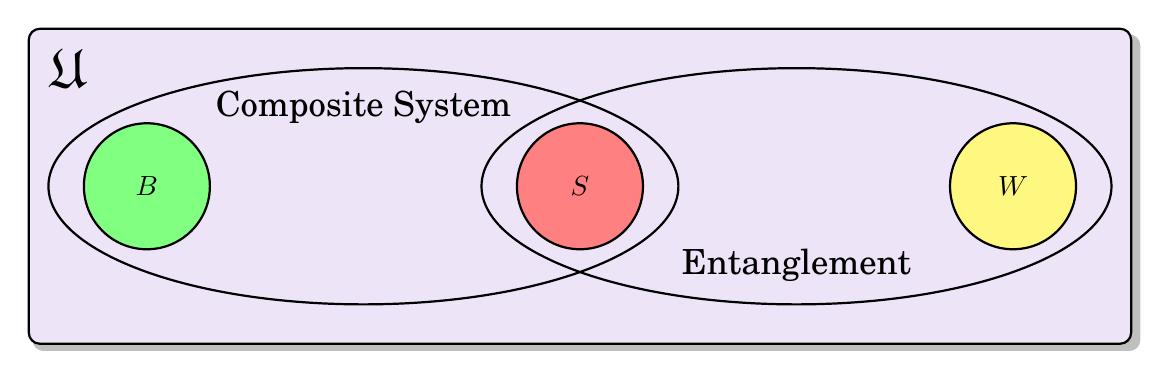
\begin{tikzpicture}[thick]
    \draw[thick, rounded corners, drop shadow={shadow scale=1.005}, fill=red!30!blue!10!white] (-8,-2) rectangle (6.0,2);
    \draw (-7.5,1.5) node[scale=2] {$\mathfrak{U}$};
    \draw[thick, fill=green!50!white] (-6.5,0) circle (0.8cm);
    \draw (-6.5,0) node[scale=1] {$B$};
    \draw[thick, fill=red!50!white] (-1.0,0) circle (0.8cm);
    \draw (-1.0,0) node[scale=1] {$S$};
    \draw[thick, fill=yellow!50!white] (4.5,0) circle (0.8cm);
    \draw (4.5,0) node[scale=1] {$W$};
    \draw[thick] (-3.75,0) ellipse (4.0cm and 1.5cm);
    \draw (-3.75,1.0) node[scale=1.25] {Composite System};
    \draw[thick] (1.75,0) ellipse (4.0cm and 1.5cm);
    \draw (1.75,-1.0) node[scale=1.25] {Entanglement};
    %
    %
\end{tikzpicture}
\end{equation}
where $\mathfrak{U}$ is the universe, $B$ is the bath, $S$ is the reduced system, and $W$ is the entanglement witness.  The entanglement witness is part of neither the reduced system nor the bath, but it is still expected that the system consisting of both $S$ and $W$ (the system ``$SW$'') must be represented by a valid density matrix.  Why is $W$ not a part of $B$?  It might be claimed that $W$ is not intended to be a physical object.  Instead, it might be argued, $W$ should just be considered a ``witness'' to the physics.  Notice, however, that the very claim of complete positivity relies on $W$ being a physical object.  

The requirement of complete positivity is a requirement of a valid (specifically positive) density matrix representation for $SW$.  If $W$ is not physical, why should $SW$ be expected to have a valid density matrix representation?  At most, it might be expected that $(SW)^\flat = S$, but notice that this is a requirement of consistency, not complete positivity.  The system $W$ has no direct correlation with the bath, but it imposes restrictions on the reduced dynamics because, as is often argued, it can never be known if the system $W$ exists or not and $S$ must always evolve into another density matrix.  It has already been pointed out that negative channels can have positivity domains that cover all of the reduced system space.  So, complete positivity is not required to insure the positivity of $S$.  

Notice also that if $B$ were maximally entangled with $S$, then the evolution of $S$ would be unaffected only if the composite dynamics were in local unitary form.  This statement would be true independently of the experimenter's knowledge of the existence of $B$.  It is implied that the reduced dynamics must be completely positive because the existence of $W$ cannot influence the channel.  The existence of $B$, however, must influence the channel.  Such logic is confusing and appears contrived.  Complete positivity is a nice property, but philosophical arguments about entanglement witnesses do not provide the sound physical motivation required to impose it on all channels as an a priori assumption.  These points were argued at the beginning of Chapter 2, but hopefully returning to them in this conclusion, after the introduction and analysis of several different negative channel examples, makes the point a little clearer. 

As a final note, it should be recognized that most of the discussion we have presented has implications far beyond quantum information theory.  Everything here was presented in the framework of quantum information theory but the conclusions extend to any open quantum system.  Complete positivity is an assumption in the field of open quantum systems and that field has been applied to everything from non-equilibrium thermodynamics to high energy physics \cite{Breuer2007}.  For example, the time inversion operator is often considered to not be physical because it is known to not be completely positive \cite{Busch1990}.    

The proposed experimental measurements of negativity we presented are not the first proposed experimental tests of complete positivity.  In the late 1990s, it was pointed out that complete positivity puts bounds on experimental parameters in both neutral kaon experiments \cite{Benatti1996} \cite{Benatti1997} \cite{Benatti1998} and neutron interferometry experiments \cite{Benatti1999}.  Experiments with neutral kaon systems were proposed as a way to test complete positivity \cite{Benatti1997a}.  The experiments we propose are much simpler (both theoretically and experimentally) and involve the concept of negativity (i.e.\ quantification of the lack of complete positivity), but the proposed neutral kaon system experiment illustrates the far reach of the complete positivity assumption.  Complete positivity has observable effects, and, if required, it limits the physical processes that are possible.  This is a limitation felt in all of theoretical physics, not just quantum information.   

There are many open questions in the study of negative channels.  Our intent is to point out that the assumption of complete positivity is not always reasonable.  Once these ideas are confirmed by experiment (e.g.\ as proposed in Section \ref{sec:proposedexp}), then the study of negative channels can be used to better understand how to implement many of the currently proposed quantum technologies, and it might even lead to new proposed technologies considered impossible under the assumption of complete positivity.


\chapter{Appendix}

\section{Discussion of the Reduced System Definition}
\label{sec:redsysdef}
The subtleties of the reduced system definition can be better understood with an example.  Consider two 2-level systems and a single particle shared between them (e.g.\ a single electron in a double quantum dot where each dot only contains two energy levels).  This system can be seen schematically in Fig.\ \ref{fig:ddqd}
\begin{figure}[th]
\centering
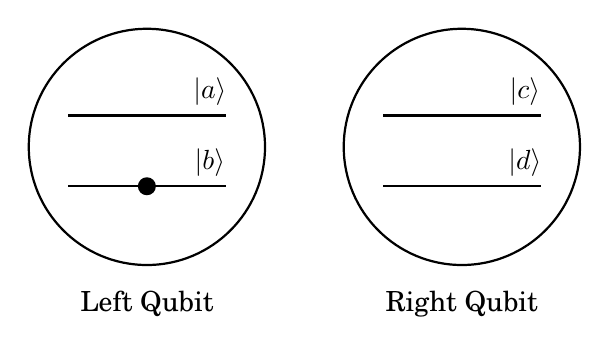
\begin{tikzpicture}
\draw [thick] (3,0.5) circle [radius=1.5];
\draw [thick] (7,0.5) circle [radius=1.5];
\draw [thick] (2.0,0.9) -- (4.0,0.9);
\draw [thick] (2.0,0.0) -- (4.0,0.0);
\draw [thick] (6.0,0.9) -- (8.0,0.9);
\draw [thick] (6.0,0.0) -- (8.0,0.0);
\draw [fill,thick] (3,0.0) circle [radius=0.1];
\node at (3,-1.5) {Left Qubit};
\node at (7,-1.5) {Right Qubit};
\node at (3.8,1.2) {$|a\rangle$};
\node at (3.8,0.3) {$|b\rangle$};
\node at (7.8,1.2) {$|c\rangle$};
\node at (7.8,0.3) {$|d\rangle$};
\end{tikzpicture}
\caption{The two level systems are spatially separated and share a single electron between them.  The electron is drawn in the lower level of the left qubit for illustrative purposes.}
\label{fig:ddqd}
\end{figure}

This example system has four energy levels, so it might feel natural to represent the system with a four dimensional Hilbert space $\mathcal{H}^T = \mathcal{H}^L\otimes\mathcal{H}^R$ where $\mathcal{H}^R$ is the two dimensional Hilbert space associated to the right dot and $\mathcal{H}^L$ is the two dimensional Hilbert space associated to the left dot.  The above definition of the reduced system implies that the right qubit can only be defined as the ``reduced system'' if it is possible to ``access'' the system with a composite operation of the form
$$
T = I\otimes U\;\;,
$$
where $I$ is the identity operator on the left qubit and $U$ is some unitary operator on the right qubit.  Mathematically, the reduced system would be defined by the partial trace over $\mathcal{H}^L$ (the partial trace will be discussed in later sections).

Notice that if the four energy levels in the system are labelled $|a\rangle$, $|b\rangle$, $|c\rangle$, and $|d\rangle$ as seen in the figure, then composite dynamics $T^\prime$ that leave the left qubit unaffected and apply $U^\prime$ to the right qubit are written in that basis as a matrix of the form
$$
T^\prime = \begin{pmatrix}
1&0&0&0\\
0&1&0&0\\
0&0&u_1^\prime&u_2^\prime\\
0&0&u_3^\prime&u_4^\prime
\end{pmatrix}
$$
where
$$
U^\prime = \begin{pmatrix}
u_1^\prime&u_2^\prime\\
u_3^\prime&u_4^\prime
\end{pmatrix}\;\;.
$$

If a ``reduced system'' exists in this system that meets the definition presented here, then there must be a basis in which $T^\prime$ can be written in the form $T$, i.e.\ $T$ must be similar to $T^\prime$ (written as $T\sim T^\prime$).  Similarity implies
$$
T = P^{-1}T^\prime P\;\;,
$$
where $P$ is some basis transformation, and
$$
\mathop{spec}\left(T\right) = \mathop{spec}\left(T^\prime\right)\;\;.
$$
The operator $T$ can be written as a matrix of the form
$$
T = \begin{pmatrix}
u_1&u_2&0&0\\
u_3&u_4&0&0\\
0&0&u_1&u_2\\
0&0&u_3&u_4
\end{pmatrix}
$$
where
$$
U = \begin{pmatrix}
u_1&u_2\\
u_3&u_4
\end{pmatrix}\;\;.
$$
Notice
$$
\mathop{spec}\left(T\right) = \left\{\lambda_+,\lambda_+,\lambda_-,\lambda_-\right\}
$$
where
$$
\mathop{spec}\left(U\right) = \left\{\lambda_+,\lambda_-\right\}\;\;,
$$
and
$$
\mathop{spec}\left(T^\prime\right) = \left\{1,1,\lambda^{\prime}_+,\lambda^{\prime}_-\right\}
$$
where
$$
\mathop{spec}\left(U^{\prime}\right) = \left\{\lambda^{\prime}_+,\lambda^{\prime}_-\right\}\;\;.
$$
As such, 
$$
T\sim T^\prime \rightarrow \lambda^{\prime}_+=\lambda^{\prime}_-\equiv \lambda^\prime\rightarrow U^\prime = \lambda^\prime I\;\;,
$$
i.e.\ if $T$ and $T^\prime$ are similar, then $U^\prime$ must be some multiple of the identity matrix.  Global phases are irrelevant in quantum mechanics, hence a multiple of the identity matrix will act the same as the identity matrix on the right qubit.  The conclusion seems to be that the given definition of the ``reduced system'' implies that the reduced system can only be formally defined for this system if the composite dynamics are trivial.

While such a conclusion may be unsatisfying, it points out the need to take care in defining the mathematical structure of the system under investigation.  If the experimenter can only access the right qubit, then the mathematical model of the composite system must reflect that in a complete way.  The desire in the construction of $T$ was ``apply $U$ to the right qubit and do nothing to the left qubit'', but a untitary $U$ that is restricted to the subspace spanned by $\{|c\rangle,|d\rangle\}$ does not consider the fact that there may be no electron in the right qubit at all.  In the mathematical model of the system presented above, if the ``reduced system'' was defined as the right qubit, then it would be possible to have a ``reduced system'' that may not contain the electron.  The ``state'' of the system is determined by which energy level is occupied by the electron, hence the ``reduced system'' could be undefined (because the only electron in the composite system may be in the ``bath'').

It may be the case that the experimenter is only able to ``access'' the right qubit for physical reasons.  The above reasoning shows that this physical situation is not described well by a 4-dimensional Hilbert space for the composite system, but that does not mean that a reduced system cannot be mathematically defined for the system.  The composite Hilbert can still be defined as $\mathcal{H}^T = \mathcal{H}^L\otimes\mathcal{H}^R$, but the subsystem Hilbert spaces $\mathcal{H}^R$ and $\mathcal{H}^L$ could be 3-dimensional (which implies $\mathcal{H}^T$ would be 9-dimensional).  The addition of a third (or ``vacuum'') energy level would account for the possibility of zero electrons in the reduced system.  The reduced system would still be defined by ``tracing out'' the Hilbert space associated to the left qubit $\mathcal{H}^L$.  There are many such ways to mathematically model a ``physical'' definition of the reduced system being just the right qubit in this system.  It is important to recognize, however, that the given definition for ``reduced system'' may require a mathematical model of the composite system that is not the most ``natural'' (or ``obvious'') choice.

To illustrate this point one more time, consider labelling the four energy levels of the above example system as $|00\rangle$, $|01\rangle$, $|10\rangle$, and $|11\rangle$.  These states span a 4-dimensional Hilbert space (which feels ``natural'' for this composite system).  Suppose, in an effort to avoid the issues involved with the first attempt at a 4-dimensional Hilbert given above, it is decided that the least significant bit in the ket notation (i.e.\ the right most number in the ket notation) represents qubit occupation (i.e.\ $0$ represents being in the right qubit and $1$ represents being in the left qubit) and the most significant bit represents energy level occupation (i.e.\ $0$ represents being in the lower energy level and $1$ represents being in the upper energy level).  The ``reduced system'' must be defined by tracing out one of the two subsystem Hilbert spaces, but tracing out the most significant bit would lead to a reduced system describing which qubit contains the electron no matter which energy level is occupied and tracing out the least significant bit would lead to a reduced system describing which energy level is occupied no matter which qubit contains the electron.  Either ``reduced system'' is mathematically well-defined, but neither is a sufficient description of the reduced system if the experimenter physically can only access the right qubit but can access each of the two energy levels in the qubit individually.

The definition of the reduced system is meant to be physical, but it must also be mathematically rigorous to avoid confusion.  The definition given here is meant to be both.  It must be kept in mind, however, that such a definition might lead to mathematical models that properly describe the physical experiment but do not ``feel natural''.  

\section{General Reduced System Dynamics}
\label{sec:genreddynamics}

The initial composite state has an eigendecomposition
$$
\left(\rho^{S}\right)^\sharp = \sum_i \lambda_i \ketbra{\Psi_i}{\Psi_i}\;\;,
$$
where $\{\lambda_i\}\in\mathbb{R}$ are the eigenvalues of $\left(\rho^{S}\right)^\sharp\in\mathcal{H}^{SB}$ and each $\ket{\Psi_i}\in\mathcal{H}^{SB}$ can be written in terms of the system and bath basis states, i.e.\ 
$$
\ket{\Psi_i} = \sum_{mn} a_{mn}^{(i)} \ket{s_m b_n}\;\;,
$$
with $\{a_{mn}\}\in\mathbb{C}$.  The states $\ket{s_m}\in\mathcal{H}^S$ and $\ket{b_n}\in\mathcal{H}^B$.  The initial composite state can then be written as
\begin{eqnarray}
\left(\rho^{S}\right)^\sharp &=& \sum_i \lambda_i \left(\sum_{mn} a_{mn}^{(i)} \ket{s_m b_n}\right)\left(\sum_{m^\prime n^\prime} a_{m^\prime n^\prime}^{(i)*} \bra{s_{m^\prime} b_{n^\prime}}\right)\\
&=& \sum_{imnm^\prime n^\prime} \lambda_i a_{mn}^{(i)}a_{m^\prime n^\prime}^{(i)*} \ketbra{s_m b_n}{s_{m^\prime} b_{n^\prime}}\\
&\equiv& \sum_{imnm^\prime n^\prime} \lambda_i a_{mn}^{(i)}a_{m^\prime n^\prime}^{(i)*} \left(\ketbra{s_m}{s_{m^\prime}} \otimes \ketbra{b_n}{b_{n^\prime}}\right)\;\;.
\end{eqnarray}
The composite evolution also has an eigendecomposition 
$$
U^{SB} = \sum_j \nu_j \ketbra{\phi_j}{\phi_j}\;\;,
$$
where $\{\nu_j\}\in\mathbb{C}$ are the eigenvalues of $U^{SB}\in\mathcal{B}(\mathcal{H}^{SB})$ and each $\ket{\phi_i}\in\mathcal{H}^{SB}$ can (again) be written in terms of the system and bath basis states, i.e.
$$
\ket{\phi_j} = \sum_{xy} c_{xy}^{(j)} \ket{s_x b_y}\;\;,
$$
with $\{c_{xy}\}\in\mathbb{C}$.  The composite evolution is then written as
\begin{eqnarray}
U^{SB} &=& \sum_{jxyx^\prime y^\prime} \nu_j c_{xy}^{(j)}c_{x^\prime y^\prime}^{(j)*} \ketbra{s_x b_y}{s_{x^\prime} b_{y^\prime}}\\
&\equiv& \sum_{jxyx^\prime y^\prime} \nu_j c_{xy}^{(j)}c_{x^\prime y^\prime}^{(j)*}\left( \ketbra{s_x}{s_{x^\prime}} \otimes \ketbra{b_y}{b_{y^\prime}}\right)\;\;.
\end{eqnarray}
Hence,
$$
\left(U^{SB}\right)^\dagger = \sum_{kopo^\prime p^\prime} \nu_k c_{op}^{(k)*}c_{o^\prime p^\prime}^{(k)} \left(|s_{o^\prime} \rangle\langle s_{o} | \otimes |b_{p^\prime} \rangle\langle b_{p} |\right)\;\;,
$$
where $\nu_k=\nu_j^*$ in the sum of $U^{SB}$.

The reduced system dynamics are then written down as 
$$
\epsilon(\rho^S) = \left((U^{SB})\left(\rho^{S}\right)^\sharp(U^{SB})^\dagger\right)^\flat  \;\;,
$$
and plugging in everything from above yields
\begin{eqnarray*}
\epsilon(\rho^S) &=& \left(\left(\sum_{jxyx^\prime y^\prime} \nu_j c_{xy}^{(j)}c_{x^\prime y^\prime}^{(j)*}\left( \ketbra{s_x}{s_{x^\prime}} \otimes \ketbra{b_y}{b_{y^\prime}}\right)\right)\right.\\
& &\left(\sum_{imnm^\prime n^\prime} \lambda_i a_{mn}^{(i)}a_{m^\prime n^\prime}^{(i)*} \left(\ketbra{s_m}{s_{m^\prime}} \otimes \ketbra{b_n}{b_{n^\prime}}\right)\right)\\
& &\left.\left(\sum_{kopo^\prime p^\prime} \nu_k c_{op}^{(k)*}c_{o^\prime p^\prime}^{(k)} \left(|s_{o^\prime} \rangle\langle s_{o} | \otimes |b_{p^\prime} \rangle\langle b_{p} |\right)\right)\right)^\flat\\
&=& \left(\sum_{\substack{jxyx^\prime \\imnm^\prime n^\prime\\kopo^\prime }} \lambda_i \nu_j \nu_k a_{mn}^{(i)}a_{m^\prime n^\prime}^{(i)*} c_{xy}^{(j)}c_{x^\prime n}^{(j)*} c_{op}^{(k)*}c_{o^\prime n^\prime}^{(k)} \left( \ket{s_x}\braket{s_{x^\prime}}{s_m}\braket{s_{m^\prime}}{s_{o^\prime}}\bra{s_{o}} \otimes \ketbra{b_y}{b_{p}}\right)\right)^\flat\\
&=& \sum_{\substack{jxyx^\prime \\imnm^\prime n^\prime\\kopo^\prime }} \lambda_i \nu_j \nu_k a_{mn}^{(i)}a_{m^\prime n^\prime}^{(i)*} c_{xy}^{(j)}c_{x^\prime n}^{(j)*} c_{op}^{(k)*}c_{o^\prime n^\prime}^{(k)} \trace\left(\ketbra{b_y}{b_{p}}\right)\left( \ket{s_x}\braket{s_{x^\prime}}{s_m}\braket{s_{m^\prime}}{s_{o^\prime}}\bra{s_{o}} \right)\\
&=& \sum_{\substack{jxyx^\prime \\imnm^\prime n^\prime\\kopo^\prime }} \lambda_i \nu_j \nu_k a_{mn}^{(i)}a_{m^\prime n^\prime}^{(i)*} c_{xy}^{(j)}c_{x^\prime n}^{(j)*} c_{op}^{(k)*}c_{o^\prime n^\prime}^{(k)} \left(\sum_q\braket{b_q}{b_y}\braket{b_{p}}{b_q}\right)\left( \ket{s_x}\braket{s_{x^\prime}}{s_m}\braket{s_{m^\prime}}{s_{o^\prime}}\bra{s_{o}} \right)\\
&=& \sum_{\substack{jxx^\prime \\imnm^\prime n^\prime\\qkoo^\prime}} \lambda_i \nu_j \nu_k a_{mn}^{(i)}a_{m^\prime n^\prime}^{(i)*} c_{xq}^{(j)}c_{x^\prime n}^{(j)*} c_{oq}^{(k)*}c_{o^\prime n^\prime}^{(k)} \left( \ket{s_x}\braket{s_{x^\prime}}{s_m}\braket{s_{m^\prime}}{s_{o^\prime}}\bra{s_{o}} \right)\\
&=& \sum_{imnm^\prime n^\prime q} \lambda_i a_{mn}^{(i)} a_{m^\prime n^\prime}^{(i)*} \hat{S}_{qn} \ketbra{s_m}{s_{m^\prime}} \hat{S}_{qn^\prime}^\dagger\;\;,
\end{eqnarray*}
where $\braket{b_{\alpha}}{b_\beta}=\delta_{\alpha\beta}$ is the delta function,
\begin{eqnarray*}
\hat{S}_{qn} &=& \sum_{jxx^\prime} \nu_j c_{xq}^{(j)} c_{x^\prime n}^{(j)*} \ketbra{s_x}{s_{x^\prime}}\\
&=& \left( I\otimes \bra{b_q}\right)U^{SB}\left(I\otimes \ket{b_n}\right)
\end{eqnarray*}
and
\begin{eqnarray*}
\hat{S}_{qn^\prime}^\dagger &=& \sum_{koo^\prime} \nu_k c_{oq}^{(k)*} c_{o^\prime n^\prime}^{(k)} \ketbra{s_{o^\prime}}{s_{o}}\\
&=& \left( I\otimes \bra{b_{n^\prime}}\right)\left(U^{SB}\right)^\dagger\left(I\otimes \ket{b_q}\right)\;\;,
\end{eqnarray*}
with $I$ as the identity on the reduced system.

\section{General Form of Initial Reduced System State}
\label{sec:genredstate}

The initial state of the reduced system must be consistent, hence
$$
\rho^S = \left((\rho^S)^\sharp\right)^\flat\;\;,
$$
where $\rho^S\in\mathcal{S}(\mathcal{H}^S)$ and $(\rho^S)^\sharp\in\mathcal{S}(\mathcal{H}^{SB})$.  The general form of the initial composite state $(\rho^S)^\sharp$ has been given in Appendix \ref{sec:genreddynamics} and can be plugged in to this consistency equation to yield
\begin{eqnarray*}
\rho^S &=& \left(\sum_{imnm^\prime n^\prime} \lambda_i a_{mn}^{(i)}a_{m^\prime n^\prime}^{(i)*} \left(\ketbra{s_m}{s_{m^\prime}} \otimes \ketbra{b_n}{b_{n^\prime}}\right)\right)^\flat\\
&=& \sum_{imnm^\prime n^\prime} \lambda_i a_{mn}^{(i)}a_{m^\prime n^\prime}^{(i)*} \trace\left(\ketbra{b_n}{b_{n^\prime}}\right)\ketbra{s_m}{s_{m^\prime}} \\
&=& \sum_{imnm^\prime n^\prime} \lambda_i a_{mn}^{(i)}a_{m^\prime n^\prime}^{(i)*} \delta_{nn^\prime}\ketbra{s_m}{s_{m^\prime}} \\
&=& \sum_{imnm^\prime} \lambda_i a_{mn}^{(i)}a_{m^\prime n}^{(i)*} \ketbra{s_m}{s_{m^\prime}} \;\;.
\end{eqnarray*}
If the initial state of the bath is some fixed pure state $\ketbra{b_n}{b_{n^\prime}}=\ketbra{b_\phi}{b_{\phi}}$, then the initial state of the reduced system becomes
$$
\rho^S = \sum_{imm^\prime} \lambda_i a_{m\phi}^{(i)}a_{m^\prime \phi}^{(i)*} \ketbra{s_m}{s_{m^\prime}}\;\;.
$$

\section{Completeness Relation for $\hat{S}_{q\phi}$}
\label{sec:Scomrelation}

From Appendix \ref{sec:genreddynamics}, the operators are given as
\begin{eqnarray*}
\hat{S}_{qn} &=& \sum_{jxx^\prime} \nu_j c_{xq}^{(j)} c_{x^\prime n}^{(j)*} \ketbra{s_x}{s_{x^\prime}}\\
&=& \left( I\otimes \bra{b_q}\right)U^{SB}\left(I\otimes \ket{b_n}\right)
\end{eqnarray*}
and
\begin{eqnarray*}
\hat{S}_{qn^\prime}^\dagger &=& \sum_{koo^\prime} \nu_k c_{oq}^{(k)*} c_{o^\prime n^\prime}^{(k)} \ketbra{s_{o^\prime}}{s_{o}}\\
&=& \left( I\otimes \bra{b_{n^\prime}}\right)\left(U^{SB}\right)^\dagger\left(I\otimes \ket{b_q}\right)\;\;.
\end{eqnarray*}
From these definitions,
\begin{eqnarray*}
\sum_q \hat{S}_{qn^\prime}^\dagger \hat{S}_{qn} &=& \sum_q \left( I\otimes \bra{b_{n^\prime}}\right)\left(U^{SB}\right)^\dagger\left(I\otimes \ket{b_q}\right)\left( I\otimes \bra{b_q}\right)U^{SB}\left(I\otimes \ket{b_n}\right)\\
&=&\sum_q \left( I\otimes \bra{b_{n^\prime}}\right)\left(U^{SB}\right)^\dagger\left(I\otimes \ketbra{b_q}{b_q}\right)U^{SB}\left(I\otimes \ket{b_n}\right)\\
&=&\left( I\otimes \bra{b_{n^\prime}}\right)\left(U^{SB}\right)^\dagger\left(I\otimes \left(\sum_q \ketbra{b_q}{b_q}\right)\right)U^{SB}\left(I\otimes \ket{b_n}\right)\\
&=& \left( I\otimes \bra{b_{n^\prime}}\right)\left(U^{SB}\right)^\dagger\left(I\otimes I\right)U^{SB}\left(I\otimes \ket{b_n}\right)\\
&=& \left( I\otimes \bra{b_{n^\prime}}\right)\left(U^{SB}\right)^\dagger U^{SB}\left(I\otimes \ket{b_n}\right)\\
&=& \left( I\otimes \bra{b_{n^\prime}}\right)\left(I\otimes \ket{b_n}\right)\\
&=& I\delta_{n^\prime n}\;\;,
\end{eqnarray*}
where $\left(U^{SB}\right)^\dagger U^{SB}=I$ by definition and $\braket{b_{n^\prime}}{b_n}=\delta_{n^\prime n}$ is the delta function.

This result can also be seen as follows:
\begin{eqnarray*}
\sum_q \hat{S}_{qn^\prime}^\dagger \hat{S}_{qn} &=& \sum_q \left(\sum_{koo^\prime} \nu_k c_{oq}^{(k)*} c_{o^\prime n^\prime}^{(k)} \ketbra{s_{o^\prime}}{s_{o}}\right)\left(\sum_{jxx^\prime} \nu_j c_{xq}^{(j)} c_{x^\prime n}^{(j)*} \ketbra{s_x}{s_{x^\prime}}\right)\\
&=& \sum_{\substack{qkoo^\prime\\jxx^\prime}} \nu_k c_{oq}^{(k)*} c_{o^\prime n^\prime}^{(k)}\nu_j c_{xq}^{(j)} c_{x^\prime n}^{(j)*} \delta_{ox} \ketbra{s_{o^\prime}}{s_{x^\prime}}\\
&=& \sum_{\substack{qko^\prime\\jxx^\prime}} \nu_k c_{xq}^{(k)*} c_{o^\prime n^\prime}^{(k)}\nu_j c_{xq}^{(j)} c_{x^\prime n}^{(j)*} \ketbra{s_{o^\prime}}{s_{x^\prime}}\\
&=& \sum_{\substack{ko^\prime\\jx^\prime}} \nu_k  c_{o^\prime n^\prime}^{(k)}\nu_j c_{x^\prime n}^{(j)*} \left(\sum_{qx} c_{xq}^{(k)*}  c_{xq}^{(j)} \right) \ketbra{s_{o^\prime}}{s_{x^\prime}}\;\;.
\end{eqnarray*}
Notice, from Appendix \ref{sec:genreddynamics},
\begin{eqnarray*}
\left(U^{SB}\right)^\dagger U^{SB} &=& \left(\sum_{kopo^\prime p^\prime} \nu_k c_{op}^{(k)*}c_{o^\prime p^\prime}^{(k)} \left(|s_{o^\prime} \rangle\langle s_{o} | \otimes |b_{p^\prime} \rangle\langle b_{p} |\right)\right)\left(\sum_{jxyx^\prime y^\prime} \nu_j c_{xy}^{(j)}c_{x^\prime y^\prime}^{(j)*}\left( \ketbra{s_x}{s_{x^\prime}} \otimes \ketbra{b_y}{b_{y^\prime}}\right)\right)\\
&=& \sum_{\substack{kopo^\prime p^\prime\\jxyx^\prime y^\prime}} \nu_k c_{op}^{(k)*}c_{o^\prime p^\prime}^{(k)}\nu_j c_{xy}^{(j)}c_{x^\prime y^\prime}^{(j)*}\delta_{ox}\delta_{py}\left(\ketbra{s_{o^\prime}}{s_{x^\prime}}\otimes\ketbra{b_{p^\prime}}{b_{y^\prime}}\right)\\
&=& \sum_{\substack{ko^\prime p^\prime\\jxyx^\prime y^\prime}} \nu_k c_{xy}^{(k)*}c_{o^\prime p^\prime}^{(k)}\nu_j c_{xy}^{(j)}c_{x^\prime y^\prime}^{(j)*}\left(\ketbra{s_{o^\prime}}{s_{x^\prime}}\otimes\ketbra{b_{p^\prime}}{b_{y^\prime}}\right)\\
\end{eqnarray*}
and
\begin{eqnarray*}
\left(\left(U^{SB}\right)^\dagger U^{SB}\right)^\flat &=&\left(\sum_{\substack{ko^\prime p^\prime\\jxyx^\prime y^\prime}} \nu_k c_{xy}^{(k)*}c_{o^\prime p^\prime}^{(k)}\nu_j c_{xy}^{(j)}c_{x^\prime y^\prime}^{(j)*}\left(\ketbra{s_{o^\prime}}{s_{x^\prime}}\otimes\ketbra{b_{p^\prime}}{b_{y^\prime}}\right)\right)^\flat\\
&=&\sum_{\substack{ko^\prime p^\prime\\jxyx^\prime y^\prime}} \nu_k c_{xy}^{(k)*}c_{o^\prime p^\prime}^{(k)}\nu_j c_{xy}^{(j)}c_{x^\prime y^\prime}^{(j)*}\delta_{p^\prime y^\prime}\ketbra{s_{o^\prime}}{s_{x^\prime}}\\
&=&\sum_{\substack{ko^\prime jx\\yx^\prime p^\prime}} \nu_k c_{xy}^{(k)*}c_{o^\prime p^\prime}^{(k)}\nu_j c_{xy}^{(j)}c_{x^\prime p^\prime}^{(j)*}\ketbra{s_{o^\prime}}{s_{x^\prime}}\\
&=& \sum_{\substack{ko^\prime j\\x^\prime p^\prime}} \nu_k c_{o^\prime p^\prime}^{(k)}\nu_j c_{x^\prime p^\prime}^{(j)*}\left(\sum_{xy} c_{xy}^{(k)*} c_{xy}^{(j)}\right) \ketbra{s_{o^\prime}}{s_{x^\prime}}\;\;.
\end{eqnarray*}
Hence,
$$
\left(\left(U^{SB}\right)^\dagger U^{SB}\right)^\flat = \sum_{p^\prime}\left(\sum_q \hat{S}_{qn^\prime}^\dagger \hat{S}_{qn}\right)\delta_{n^\prime p^\prime}\delta_{np^\prime} = \sum_{n}\left(\sum_q \hat{S}_{qn^\prime}^\dagger \hat{S}_{qn}\right)\delta_{n^\prime n}\;\;.
$$
Notice
$$
\left(U^{SB}\right)^\dagger U^{SB} = I\in\mathcal{H}^{SB}\Rightarrow \left(\left(U^{SB}\right)^\dagger U^{SB}\right)^\flat = I\in\mathcal{B}(\mathcal{H}^S)\;\;,
$$
where $I$ is the identity operator, which implies
$$
\sum_{nq} \hat{S}_{qn^\prime}^\dagger \hat{S}_{qn}\delta_{n^\prime n} = I\;\;.
$$
This relation is expected from the definition of the operators $\hat{S}_{qn}$ as the re-stacked Choi representation of the channel, which is a Hermitian matrix \cite{Choi1975}.

If the bath is in some specific pure state $\ketbra{b_n}{b_{n^\prime}}=\ketbra{b_\phi}{b_{\phi}}$, then there is no sum over the bath states.  In such a case,
$$
\sum_{q} \hat{S}_{q\phi}^\dagger \hat{S}_{q\phi} = I\;\;.
$$

\section{Rabi Model Derivation}
\label{sec:rabimodelder}

Maxwell's equations relate the electric and magnetic fields, $\mathbf{E}$ and $\mathbf{B}$, to the charge density $\varrho$ and the current density $\mathbf{j}$ \cite{Cohen1997}.  They are
\begin{eqnarray*}
\nabla\cdot \mathbf{E}(\mathbf{r},t) &=& \frac{\varrho(\mathbf{r},t)}{\epsilon_0}\\
\nabla\cdot \mathbf{B}(\mathbf{r},t) &=& 0\\
\nabla\times \mathbf{E}(\mathbf{r},t) &=& -\frac{\partial}{\partial t}\mathbf{B}(\mathbf{r},t)\\
\nabla\times \mathbf{B}(\mathbf{r},t) &=& \frac{1}{c^2}\frac{\partial}{\partial t}\mathbf{E}(\mathbf{r},t)+\frac{\mathbf{j}(\mathbf{r},t)}{\epsilon_0 c^2}\;\;,\\
\end{eqnarray*}
where the constant $c$ is the speed of light in a vacuum and the constant $\epsilon_0$ is the vacuum permittivity.  The dependence on the position vector $\mathbf{r}$ and time $t$ has been written explicitly for the electric and magnetic field vectors, the current density vector, and the charge density.  The middle two equations from above suggest the following forms for the electric and magnetic fields:
\begin{eqnarray*}
\mathbf{B}(\mathbf{r},t) &=& \nabla\times \mathbf{A}(\mathbf{r},t)\\
\mathbf{E}(\mathbf{r},t) &=& -\frac{\partial}{\partial t}\mathbf{A}(\mathbf{r},t) - \nabla\Phi(\mathbf{r},t)\;\;,
\end{eqnarray*}
where $\mathbf{A}$ is called the ``vector potential field'' and $\Phi$ is called the ``scalar potential field''.  

The Lorentz force law is
$$
\mathbf{F} = q\mathbf{E}+q\left(\mathbf{v}\times\mathbf{B}\right)
$$
where $q$ is the electric charge of a particle moving with velocity $\mathbf{v}$ through the electric and magnetic fields $
\mathbf{E}$ and $\mathbf{B}$.  The time and space dependence of the fields is left out of these expressions for clarity of presentation, but it should be remembered that those dependences are still implied.  This expression can be written in terms of the potentials as
$$
\mathbf{F} = q\left(-\nabla\Phi + \nabla\left(\mathbf{v}\cdot\mathbf{A}\right)-\frac{d}{dt}\mathbf{A}\right)
$$
where the the vector identity (for some vectors $\mathbf{K_1}$ and $\mathbf{K_2}$)
$$
\mathbf{K_1} \times \left(\nabla\times \mathbf{K_2}\right) = \nabla\left(\mathbf{K_1}\cdot\mathbf{K_2}\right)-\left(\mathbf{K_1}\cdot\nabla\right)\mathbf{K_2}-\left(\mathbf{K_2}\cdot\nabla\right)\mathbf{K_1}-\mathbf{K_2}\times\left(\nabla\times\mathbf{K_1}\right)
$$
is used along with the fact that $\nabla\mathbf{v}=0$ and $\nabla\times\mathbf{v}=\mathbf{0}$ to yield
$$
\mathbf{v}\times \left(\nabla\times \mathbf{A}\right) = \nabla\left(\mathbf{v}\cdot\mathbf{A}\right)-\left(\mathbf{v}\cdot\nabla\right)\mathbf{A}\;\;,
$$
which can be rewritten by recognizing
$$
\frac{d}{dt}\mathbf{A} = \frac{\partial}{\partial t}\mathbf{A}+\frac{\partial}{\partial x}\mathbf{A}\frac{d}{dt}x+\frac{\partial}{\partial y}\mathbf{A}\frac{d}{dt}y+\frac{\partial}{\partial z}\mathbf{A}\frac{d}{dt}z=\frac{\partial}{\partial t}\mathbf{A}+\left(\mathbf{v}\cdot\nabla\right)\mathbf{A}\;\;.
$$

The system under investigation will be assumed to be conservative (i.e.\ $\mathbf{F} = -\nabla V$ where $V$ is the potential energy), which allows us the write the potential energy as
$$
V = q\Phi - q\left(\mathbf{v}\cdot\mathbf{A}\right)\;\;.
$$
The kinetic energy of the system is given by
$$
T = \frac{m\mathbf{v}\cdot\mathbf{v}}{2}\;\;,
$$
which implies the (classical) electromagnetic Lagrangian is
$$
L = T-V = \frac{m\mathbf{v}\cdot\mathbf{v}}{2} - q\Phi + q\left(\mathbf{v}\cdot\mathbf{A}\right)\;\;.
$$ 
The canonical momentum
$$
\mathbf{p} = \frac{\partial}{\partial\mathbf{v}}L = m\mathbf{v}+q\mathbf{A}
$$
leads to the (classical) electromagnetic Hamiltonian
$$
H = \mathbf{p}\cdot\mathbf{v}-L = \frac{1}{2m}\left(\mathbf{p}-q\mathbf{A}(\mathbf{r},t)\right)^2+q\Phi(\mathbf{r},t)\;\;,
$$
where the explicit dependence of the potentials on position and time has again been added for emphasis.  Notice that this Hamiltonian is for a single particle with a potential governed solely by the electromagnetic field (i.e.\ there are no other potentials in this system).

In standard quantum mechanics, the correspondence principle is used to form a quantum Hamiltonian from the above classical one.  The operators that satisfy the canonical commutation relations are $\hat{\mathbf{r}}$ and $\hat{\mathbf{p}} = -i\hbar\nabla$ (see \cite{Cohen1997} for a discussion of these points with respect to the electromagnetic Hamiltonian).  Using this substitution, the quantum Hamiltonian can immediately be written down as
$$
H_e = \frac{1}{2m}\left(-i\hbar\nabla-e\hat{\mathbf{A}}(\hat{\mathbf{r}},t)\right)^2 -e\Phi(\hat{\mathbf{r}},t)\;\;,
$$
where we have assumed that the charged particle is an electron, i.e.\ $q=e$ where $e$ as the charge of the electron.  

The classical fields are said to invariant under ``gauge transformations'' of the form
\begin{eqnarray*}
\mathbf{A}\left(\mathbf{r},t\right)&\rightarrow & \mathbf{A}^\prime\left(\mathbf{r},t\right)=\mathbf{A}\left(\mathbf{r},t\right)+\nabla F\left(\mathbf{r},t\right)\\
\Phi\left(\mathbf{r},t\right) &\rightarrow & \Phi^\prime\left(\mathbf{r},t\right) = \Phi\left(\mathbf{r},t\right) - \frac{\partial}{\partial t} F\left(\mathbf{r},t\right)\;\;,
\end{eqnarray*}
where $F\left(\mathbf{r},t\right)$ is an arbitrary function of the position and time.  The idea is that the same fields $\mathbf{E}$ and $\mathbf{B}$ can be described by either $\mathbf{A}\left(\mathbf{r},t\right)$ and $\Phi\left(\mathbf{r},t\right)$ or $\mathbf{A}^\prime\left(\mathbf{r},t\right)$ and $\Phi^\prime\left(\mathbf{r},t\right)$.  This freedom can be useful in working through the above equations.  The ``Coulomb'' (or radiation \cite{Cohen1997}) gauge is the condition
$$
\nabla\cdot\mathbf{A}\left(\mathbf{r},t\right)=0\;\;.
$$
Applying this gauge to the quantum electromagnetic Hamiltonian yields
$$
H_e = -\frac{\hbar^2}{2m}\nabla^2 + \frac{i\hbar e}{m}\hat{\mathbf{A}}\left(\hat{\mathbf{r}},t\right)\cdot\nabla+\frac{e^2}{2m}\hat{\mathbf{A}}^2\left(\hat{\mathbf{r}},t\right)-e\Phi(\hat{\mathbf{r}},t)\;\;.
$$
The scalar potential can be set to zero (sometimes referred to as the ``velocity gauge'' \cite{Faisal1987}), and we can assume the fields are ``weak'' in the sense that the terms proportional to the square of the vector potential can be ignored\footnote{See pages 688-689 in \cite{Mandel1995} for a discussion of why the assumption of ``weak'' fields is reasonable ``for all but the most intense optical fields''.}.  These assumptions lead to
$$
H_e \approx -\frac{\hbar^2}{2m}\nabla^2 + \frac{i\hbar e}{m}\hat{\mathbf{A}}\left(\hat{\mathbf{r}},t\right)\cdot\nabla\;\;.
$$

Ehrenfest's theorem \cite{Schwabl2007} states 
$$
\frac{d}{dt}\mean{O} = \frac{i}{\hbar}\mean{[H,O]}+\mean{\frac{\partial }{\partial t}O}
$$ for some operator $O$.  In particular, for the position operator, 
$$
\frac{d}{dt}\mean{\hat{\mathbf{r}}} = \frac{i}{\hbar}\mean{[H,\hat{\mathbf{r}}]}+\mean{\frac{\partial }{\partial t}\hat{\mathbf{r}}}\;\;.
$$  
The position operator does not explicitly depend on time, so this equation reduces to 
$$
\frac{d}{dt}\mean{\hat{\mathbf{r}}} = \frac{i}{\hbar}\mean{[\frac{\hat{\mathbf{p}}^2}{2m}+V(\hat{\mathbf{r}}),\hat{\mathbf{r}}]}
$$ 
where the Hamiltonian operator has been written out in terms of the potential and momentum as $H=\frac{\hat{\mathbf{p}}^2}{2m}+V(\hat{\mathbf{r}})$.  Notice $\mean{[V(\hat{\mathbf{r}}),\hat{\mathbf{r}}]}=0$, so everything can be further reduced: 
\begin{eqnarray*}
\frac{d}{dt}\mean{\hat{\mathbf{r}}} &=& \frac{i}{\hbar}\mean{[\frac{\hat{\mathbf{p}}^2}{2m},\hat{\mathbf{r}}]}\\
&=& \frac{i}{2m\hbar}\mean{[\hat{\mathbf{p}}^2,\hat{\mathbf{r}}]}\\
&=& \frac{i}{2m\hbar}\mean{\hat{\mathbf{p}}[\hat{\mathbf{p}},\hat{\mathbf{r}}]+[\hat{\mathbf{p}},\hat{\mathbf{r}}]\hat{\mathbf{p}}}\\
&=&-\frac{i}{2m\hbar}\mean{\hat{\mathbf{p}}i\hbar+i\hbar \hat{\mathbf{p}}}\\
&=& \frac{2\hbar}{2m\hbar}\mean{\hat{\mathbf{p}}}\\
&=& \frac{\mean{\hat{\mathbf{p}}}}{m}\;\;.
\end{eqnarray*}
This result implies 
$$
\mean{\hat{\mathbf{p}}}=m\frac{d\mean{\hat{\mathbf{r}}}}{dt}\;\;,
$$
and this final result will be used as a justification for making the substitution $-i\hbar\nabla\rightarrow m\frac{d\hat{\mathbf{r}}}{dt}$, which is referred to as the ``time-dependent form'' of the momentum operator.  Making this substitution yields
$$
H_e \approx -\frac{\hbar^2}{2m}\nabla^2 + e\hat{\mathbf{A}}\left(\hat{\mathbf{r}},t\right)\cdot\frac{d}{dt}\hat{\mathbf{r}}\;\;.
$$
Notice
$$
\hat{\mathbf{A}}(\hat{\mathbf{r}},t)\cdot\frac{d\hat{\mathbf{r}}}{dt} = \frac{d}{dt}\left(\hat{\mathbf{A}}(\hat{\mathbf{r}},t)\cdot\hat{\mathbf{r}}\right)-\frac{d\hat{\mathbf{A}}(\hat{\mathbf{r}},t)}{dt}\cdot\hat{\mathbf{r}} \;\;,
$$
which leads to
$$
H_e \approx -\frac{\hbar^2}{2m}\nabla^2 +e\left(\frac{d}{dt}\left(\hat{\mathbf{A}}(\hat{\mathbf{r}},t)\cdot\hat{\mathbf{r}}\right)-\frac{d\hat{\mathbf{A}}(\hat{\mathbf{r}},t)}{dt}\cdot\hat{\mathbf{r}}\right)\;\;.
$$

At this point it will be further assumed that the electromagnetic field has no spatial variation across the qubit.  This is the assumption that the position operator $\hat{\mathbf{r}}$ in the potentials can be treated as a constant and replaced by its average value $\mathbf{r}_0$.  Specifically, $\hat{\mathbf{A}}\left(\hat{\mathbf{r}},t\right)\rightarrow \mathbf{A}\left(\mathbf{r}_0,t\right)$.  This assumption is referred to as the ``dipole approximation''.

Consider a specific form of the classical vector potential given as
$$
\mathbf{A}(\mathbf{r},t)=\frac{1}{2}\left(\mathbf{B}(t)\times\mathbf{r}\right)\;\;.
$$
where the magnetic field does not explicitly depend on position.  The vector identity (for some vectors $\mathbf{K_1}$ and $\mathbf{K_2}$)
$$
\nabla\times\left(\mathbf{K_1}\times\mathbf{K_2}\right) = \mathbf{K_1}\left(\nabla\cdot\mathbf{K_2}\right)-\mathbf{K_2}\left(\nabla\cdot\mathbf{K_1}\right)+\left(\mathbf{K_2}\cdot\nabla\right)\mathbf{K_1}-\left(\mathbf{K_1}\cdot\nabla\right)\mathbf{K_2}\;\;,
$$
along with the fact that $\nabla\cdot\mathbf{r}=3$ and $\nabla\mathbf{r}=1$, implies
$$
\nabla\times\mathbf{A}(\mathbf{r},t) = \mathbf{B}(t)
$$
as desired.  The vector identities
$$
\nabla\cdot\left(\mathbf{K_1}\times\mathbf{K_2}\right) = \mathbf{K_2}\cdot\left(\nabla\times\mathbf{K_1}\right)-\mathbf{K_1}\cdot\left(\nabla\times\mathbf{K_2}\right)
$$
and
$$
\nabla\times\left(\nabla\times\mathbf{K_1}\right) = \nabla\left(\nabla\cdot\mathbf{K_1}\right)-\nabla^2\mathbf{K_1}
$$
imply
$$
\nabla\cdot\mathbf{A}(\mathbf{r},t) = 0
$$
because $\nabla^2\mathbf{A}(\mathbf{r},t)=0$ in the dipole approximation and we are working in the Coulomb gauge (which is consistent with the above result).  It follows that this specific form of the vector potential is valid in the Coulomb gauge given the dipole approximation.

The first vector potential term in the Hamiltonian can be shown to be zero after applying the dipole approximation and the above form of the vector potential, i.e.\
$$
\frac{d}{dt}\left(\mathbf{A}(\mathbf{r}_0,t)\cdot\hat{\mathbf{r}}\right) = 0
$$
where we have used the $\mathbf{K_1}\cdot\mathbf{K_2}=\mathbf{K_2}\cdot\mathbf{K_1}$ property of the scalar product, the triple scalar product rule (i.e.\ $\mathbf{K_1}\cdot\left(\mathbf{K_2}\times\mathbf{K_3}\right)=\mathbf{K_2}\cdot\left(\mathbf{K_3}\times\mathbf{K_1}\right)=\mathbf{K_3}\cdot\left(\mathbf{K_1}\times\mathbf{K_2}\right)$ for some vectors $\mathbf{K_1}$, $\mathbf{K_2}$, and $\mathbf{K_3}$), and the fact that $\mathbf{r}\times\mathbf{r}=0$.

The other vector potential term in the Hamiltonian can also be reduced using the dipole approximation and remembering that the scalar potential has already been assumed to be zero.  As such, the electric field is given only by the negative time derivative of the vector potential and
$$
-\frac{d\mathbf{A}(\mathbf{r}_0,t)}{dt}\cdot\hat{\mathbf{r}} = e\mathbf{E}\left(\mathbf{r}_0,t\right)\cdot\hat{\mathbf{r}}\;\;.
$$

The final approximate Hamiltonian is
$$
H_e = -\frac{\hbar^2}{2m}\nabla^2+e\mathbf{E}(\mathbf{r}_0,t)\cdot\hat{\mathbf{r}} = H_f + H_{di}\;\;,
$$
where the Hamiltonian is explicitly split into two terms in the last step with
$$
H_{di} \equiv e\mathbf{E}(\mathbf{r}_0,t)\cdot\hat{\mathbf{r}}
$$
and
$$
H_f \equiv -\frac{\hbar^2}{2m}\nabla^2
$$
to emphasize that the Hamiltonian is just the free particle Hamiltonian with a ``dipole term'' added.

The dipole Hamiltonian can be written as
$$
H_{di} = -\mathbf{E}(\mathbf{r}_0,t)\cdot\hat{\mathbf{D}}
$$
where the dipole operator is defined as $\hat{\mathbf{D}}=-e\hat{\mathbf{r}}$.  Although this notation is not used much in our work, it is the standard notation of the dipole interaction Hamiltonian in most derivations \cite{Loudon2000,Mandel1995,Cohen1997}.

We will now consider a two level system with energy levels labelled $\ket{0}$ and $\ket{1}$ that have associated energy eigenvalues of $-\hbar\omega_0/2$ and $\hbar\omega_0/2$ respectively.  The system interacts with an electromagnetic field that is propagating in the direction $\mathbf{n}$, oscillates with a frequency $\omega$, and has a polarization of $\mathbf{\epsilon}$, which can be described as
$$
\mathbf{E}(\mathbf{r}_0,t) = E_0\left( \mathbf{\epsilon} e^{i\left(\omega t-(\mathbf{k}\cdot\mathbf{n}) |\mathbf{r}_0|\right)} + \mathbf{\epsilon}^* e^{-i\left(\omega t-(\mathbf{k}\cdot\mathbf{n}) |\mathbf{r}_0|\right)}\right)\;\;,
$$
where $E_0\in\mathbb{R}$ is the amplitude of the field.  It can be assumed that the two level system is located at the origin.  Therefore, $|\mathbf{r}_0|=0$, and the second terms in the exponentials vanish leaving only
$$
\mathbf{E}(t) = E_0\left( \mathbf{\epsilon} e^{i\omega t} + \mathbf{\epsilon}^* e^{-i\omega t}\right)\;\;.
$$
This field can be used to write down the final approximate Hamiltonian in matrix form.  

The first step is to find the off-diagonal terms of the dipole Hamiltonian $H_{di}$ as
\begin{eqnarray*}
\bra{1}H_{di}\ket{0} &=& \bra{1}\left(e\mathbf{E}(t)\cdot\hat{\mathbf{r}}\right)\ket{0} = e E_0 \hat{\mathbf{r}}_{10}\cdot\left(\mathbf{\epsilon} e^{i\omega t} + \mathbf{\epsilon}^* e^{-i\omega t}\right)\;\;,
\end{eqnarray*}
with $\hat{\mathbf{r}}_{10} = \bra{1}\hat{\mathbf{r}}\ket{0}$.  The Hamiltonian is Hermitian by definition, hence $\bra{0}H_{di}\ket{1} = (\bra{1}H_{di}\ket{0})^*$. In general, $\bra{0}H_{di}\ket{1}$ is a complex quantity \cite{Faisal1987}, but it will be real for transitions between bound states \cite{Loudon2000} (where the states $\ket{0}$ and $\ket{1}$ are real), which is precisely the situation we wish to model in this derivation.  As such, we will use $\bra{0}H_{di}\ket{1} = \bra{1}H_{di}\ket{0}$ and ignore the customary explicit conjugation notation in the Hamiltonians that follow.

The position operator $\hat{\mathbf{r}}$ has odd parity.  To see this fact, define the parity operator $\hat{\mathbf{P}}$ by its action on the position state of a system: $\hat{\mathbf{P}}\ket{r} = \ket{-r}$ and $\bra{r}\hat{\mathbf{P}}^\dagger = \bra{-r}$.  Notice $\hat{\mathbf{P}}^2=\hat{\mathbf{P}}^\dagger\hat{\mathbf{P}}=\hat{\mathbf{P}}\hat{\mathbf{P}}^\dagger=I$ (where $I$ is the identity operator) and $\hat{\mathbf{P}}=\hat{\mathbf{P}}^\dagger$.  The position operator $\hat{\mathbf{r}}$ is defined by $\hat{\mathbf{r}}\ket{r}=r^\prime\ket{r}$ which implies
\begin{eqnarray*}
\hat{\mathbf{P}}\hat{\mathbf{r}}\hat{\mathbf{P}}\ket{r}&=&\hat{\mathbf{P}}\hat{\mathbf{r}}\ket{-r}\\
&=&\hat{\mathbf{P}}(-r^\prime)\ket{-r}\\
&=&(-r^\prime)\ket{r}\\
&=&-(\hat{\mathbf{r}}\ket{r})\;\;.
\end{eqnarray*}
Therefore, $\hat{\mathbf{r}}$ has odd parity.  This result implies
\begin{eqnarray*}
\bra{0}\hat{\mathbf{r}}\ket{0}&=&\bra{0}\hat{\mathbf{P}}^\dagger\hat{\mathbf{P}}\hat{\mathbf{r}}\hat{\mathbf{P}}^\dagger\hat{\mathbf{P}}\ket{0}\\
&=&-\bra{0}\hat{\mathbf{P}}^\dagger\hat{\mathbf{r}}\hat{\mathbf{P}}\ket{0}\\
&=&-\bra{0}\hat{\mathbf{r}}\ket{0}
\end{eqnarray*} 
because the parity of the state $\ket{0}$ is either even or odd (i.e.\ the state $\ket{0}$ is an eigenstate of the parity operator with an eigenvalue of either $+1$ or $-1$).  The final implication is that $\bra{0}\hat{\mathbf{r}}\ket{0}=0$.  Similarly, $\bra{1}\hat{\mathbf{r}}\ket{1}=0$.  This result, in turn, implies $\bra{0}H_{di}\ket{0}=\bra{1}H_{di}\ket{1}=0$; hence, there are no diagonal terms for $H_{di}$.

Putting everything together yields the matrix form of the final approximate Hamiltonian as \cite{Kok2010}
$$
H_e = \begin{pmatrix}
-\frac{\hbar \omega_o}{2} & e E_0 \hat{\mathbf{r}}_{10}\cdot\left(\mathbf{\epsilon} e^{i\omega t} + \mathbf{\epsilon}^* e^{-i\omega t}\right)\\
e E_0 \hat{\mathbf{r}}_{10}\cdot\left(\mathbf{\epsilon} e^{i\omega t} + \mathbf{\epsilon}^* e^{-i\omega t}\right) & \frac{\hbar \omega_o}{2}
\end{pmatrix}\;\;.
$$
Several approximations have already been applied to derive this Hamiltonian, but it is still too complicated to solve Schr\"{o}dinger's equation directly because of the time dependence in the off-diagonal terms.  As a final step, we apply the rotating wave approximation to yield a Hamiltonian more amenable to theoretical investigation.

The first step is to transform the wavefunction to a frame that rotates at the frequency of the optical field (i.e.\ $\omega$) using
$$
U = \operatorname{diag}\left(e^{i\omega t/2},e^{-i\omega t/2}\right)\;\;.
$$
The wavefunction in this new frame is defined as $\ket{\psi^\prime}=U\ket{\psi}$ (or $\ket{\psi}=U^\dagger \ket{\psi^\prime}$) and Schr\"{o}dinger's equation becomes
\begin{eqnarray*}
H_e \ket{\psi} = -i\hbar\frac{d}{dt}\ket{\psi}\rightarrow H_e U^\dagger\ket{\psi^\prime} &=& -i\hbar\frac{d}{dt}\left(U^\dagger \ket{\psi^\prime}\right)\\
&=& -i\hbar U^\dagger \frac{d}{dt}\ket{\psi^\prime}-i\hbar\left(\frac{d}{dt}U^\dagger\right)\ket{\psi^\prime}\;\;,
\end{eqnarray*}
which can be multiplied by $U$ (and rearranged) to yield
\begin{eqnarray*}
\left(UH_eU^\dagger+i\hbar U\frac{d}{dt}U^\dagger\right)\ket{\psi^\prime}&=&-i\hbar\frac{d}{dt}\ket{\psi^\prime}\\
H_e^\prime \ket{\psi^\prime} &=& -i\hbar\frac{d}{dt}\ket{\psi^\prime}
\end{eqnarray*}
where the new ``rotated'' Hamiltonian can now be written down directly as
\begin{eqnarray*}
H_e^\prime &=& \left(UH_eU^\dagger+i\hbar U\frac{d}{dt}U^\dagger\right)\\
&=& \begin{pmatrix}
-\frac{\hbar(\omega_o-\omega)}{2} & e E_0\mathbf{r}_{10}\cdot\left(\mathbf{\epsilon}+\mathbf{\epsilon}^*e^{2i\omega t}\right)\\
e E_0\mathbf{r}_{10}\cdot\left(\mathbf{\epsilon}+\mathbf{\epsilon}^*e^{-2i\omega t} \right)& \frac{\hbar(\omega_o-\omega)}{2}
\end{pmatrix}\;\;.
\end{eqnarray*}
The final assumption in this derivation is to assume that the external field is close to resonance with the energy gap of the atom, i.e.\ $(\omega-\omega_0)<<\omega$ and $E_0<<\omega$, which means the fast oscillating term of $e^{2i\omega t}$ can be ignored in the Hamiltonian.  All of this work leads to 
\begin{eqnarray*}
H_e^\prime &=& \begin{pmatrix}
-\frac{\hbar(\omega_o-\omega)}{2} & e E_0\left(\mathbf{r}_{10}\cdot\mathbf{\epsilon}\right)\\
e E_0\left(\mathbf{r}_{10}\cdot\mathbf{\epsilon}\right)& \frac{\hbar(\omega_o-\omega)}{2}
\end{pmatrix}\\
&=& \frac{\hbar}{2}\begin{pmatrix}
-\nu & \Omega\\
\Omega & \nu
\end{pmatrix}\;\;,
\end{eqnarray*}
where
$$
\nu \equiv \omega_o-\omega
$$
is called the detuning and
$$
\Omega \equiv \frac{2eE_0\left(\mathbf{r}_{10}\cdot\mathbf{\epsilon}\right)}{\hbar}
$$
is called the Rabi frequency.  Notice that the Rabi frequency is always real in our derivation.  This model of an atom is called the Rabi model, and it is a common model used in theoretical descriptions of nuclear magnetic resonance (NMR) and other quantum information experiments \cite{Mikio2008}.


\bibliographystyle{abbrv}
\bibliography{ThesisNotes_GMUFormat}




\end{document}